\documentclass[handout,10pt]{beamer}
\usepackage{SexySlides1,fancyvrb,outlines,pbox}
\usepackage[round]{natbib}
\usepackage{hyperref} % link references
\usepackage[font=footnotesize]{caption} % caption options
\usepackage{fancyvrb}

\usepackage[tikz]{bclogo}
\presetkeys{bclogo}{
ombre=true,
epBord=3,
couleur = white,
couleurBord = black,
arrondi = 0.2,
logo=\bctrombone
}{}

\definecolor{UniBlue}{RGB}{83,121,170}
\setbeamercolor{title}{fg=UniBlue}
\setbeamercolor{frametitle}{fg=UniBlue}
\newcommand{\coluit}{\color{UniBlue}\it}
\newcommand{\colubf}{\color{UniBlue}\bf}
\DeclareMathOperator*{\diag}{diag}
\DeclareMathOperator*{\Tr}{Tr}
\DeclareMathOperator*{\argmin}{argmin}

% Row color change in table
\makeatletter
\def\zapcolorreset{\let\reset@color\relax\ignorespaces}
\def\colorrows#1{\noalign{\aftergroup\zapcolorreset#1}\ignorespaces}
\makeatother

     \setbeamertemplate{footline}
        {
      \leavevmode%
      \hbox{%
      \begin{beamercolorbox}[wd=.333333\paperwidth,ht=2.25ex,dp=1ex,center]{author in head/foot}%
        \usebeamerfont{author in head/foot}\insertshortauthor~~
        %(\insertshortinstitute)
      \end{beamercolorbox}%
      \begin{beamercolorbox}[wd=.333333\paperwidth,ht=2.25ex,dp=1ex,center]{title in head/foot}%
        \usebeamerfont{title in head/foot}\insertshorttitle
      \end{beamercolorbox}%
      \begin{beamercolorbox}[wd=.333333\paperwidth,ht=2.25ex,dp=1ex,right]{date in head/foot}%
        \usebeamerfont{date in head/foot}\insertshortdate{}\hspace*{2em}

    %#turning the next line into a comment, erases the frame numbers
        %\insertframenumber{} / \inserttotalframenumber\hspace*{2ex} 

      \end{beamercolorbox}}}%

%\def\logo{%
%{\includegraphics[height=1cm]{goldy1.png}}
%}
%%
%\setbeamertemplate{footline}
%{%
%	\hspace*{.05cm}\logo
%  \begin{beamercolorbox}[sep=1em,wd=10cm,rightskip=0.5cm]
%  {footlinecolor,author in head/foot}
%%    \usebeamercolor{UniBlue}
%    \vspace{0.1cm}
%    \insertshortdate \hfill \insertshorttitle
%    \newline
%    \insertshortauthor   - \insertshortinstitute
%    \hfill
%    \hfill \insertframenumber/\inserttotalframenumber
%  \end{beamercolorbox}
%  \vspace*{0.05cm}
%}

%% smart verbatim
\fvset{framesep=1cm,fontfamily=courier,fontsize=\scriptsize,framerule=.3mm,numbersep=1mm,commandchars=\\\{\}}

\title[Depth-based Inference]
{\Large  
An Inferential Perspective on Data Depth}

\author[Subho Majumdar]{Subhabrata Majumdar}
\institute[]{under supervision of\\
Snigdhansu Chatterjee\\
University of Minnesota, School of Statistics\\
\vspace{1em}
May 18, 2017} 

%\vspace{.5cm}
%\includegraphics[height=.5cm]{UMNlogo}}

\date [May 18, 2017]

%%%%%%%List Outline in the beginning of each section.
\AtBeginSection[] {
   \begin{frame}
       \frametitle{Outline}
       \tableofcontents[currentsection]
   \end{frame}
}

%-------------------------------------------------------------------
\begin{document}

%\begin{frame}
%%%%%%%%%%%%%%%%%%%%%%%%%%%%%%%%%%%%%%%%%%%%%%%%%%%%%%%%%%%%%%%

\frame{ \titlepage}

%%%%%%%%%%%%%%%%%%%%%%%%%%%%%%%%%%%%%%%%%%%%%%%%%%%%%%%%%%%%%%%

\frame{\frametitle{Table of contents}\tableofcontents}

%%%%%%%%%%%%%%%%%%%%%%%%%%%%%%%%%%%%%%%%%%%%%%%%%%%%%%%%%%%%%%%

% Section 1: background
\section{Introduction}
%%%%%%%%%%%%%%%%%%%%%%%%%%%%%%%%%%%%%%%%%%%%%%%%%%%%%%%%%%%%%%%%

\begin{frame}
\frametitle{What is depth?}
\textbf{Example}: 500 points from $\mathcal{N}_2 ((0,0)^T, \diag (2,1))$
\begin{figure}\begin{center}
   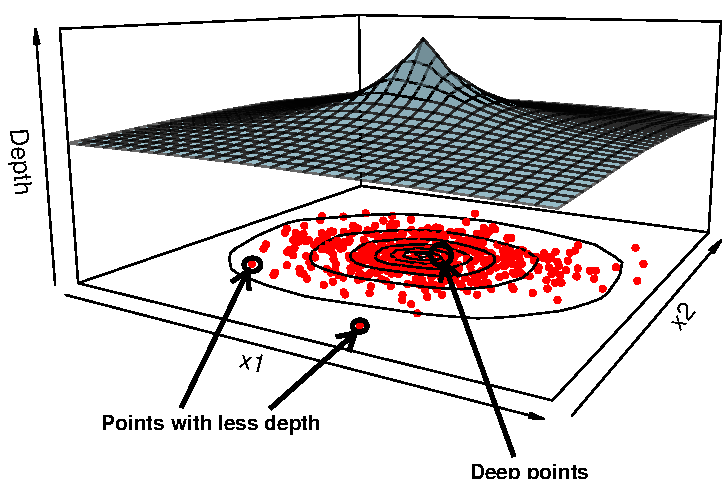
\includegraphics[height=6cm]{depthplot_cropped}
   \label{fig:fig1}
\end{center}\end{figure}
\colbbf{A scalar measure of how much inside a point is with respect to a data cloud}
\end{frame}

%%%%%%%%%%%%%%%%%%%%%%%%%%%%%%%%%%%%%%%%%%%%%%%%%%%%%%%%%%%%%%%

\begin{frame}
\frametitle{Formal definition of depth}
For any multivariate distribution $F = F_\bfX$, the depth of a point $\bfx \in \mathbb{R}^p$, say $D(\bfx, F_\bfX)$ is any real-valued function that provides a `center outward ordering' of $\bfx$ with respect to $F$ \citep{zuo00}.

\vspace{.5cm}
\begin{block}{Desirable properties \citep{liu90}}
(P1) {\colbit Affine invariance}: $D(A\bfx + \bfb, F_{A\bfX+\bfb}) = D(\bfx, F_\bfX)$
\vspace{.2cm}

(P2) {\colbit Maximality at center}: $D(\bftheta, F_\bfX) = \sup_{\bfx\in \mathbb{R}^p} D(\bfx, F_\bfX)$ for $F_\bfX$ with center of symmetry $\bftheta$, the \textit{deepest point} of $F_\bfX$.
\vspace{.2cm}

(P3) {\colbit Monotonicity w.r.t. deepest point}: $D(\bfx; F_\bfX) \leq D(\bftheta + a(\bfx - \bftheta), F_\bfX)$
\vspace{.5cm}

(P4) {\colbit Vanishing at infinity}: $D(\bfx; F_\bfX) \rightarrow \bf0$ as $\|\bfx\| \rightarrow \infty $.
\end{block}
\end{frame}

%%%%%%%%%%%%%%%%%%%%%%%%%%%%%%%%%%%%%%%%%%%%%%%%%%%%%%%%%%%%%%%

\begin{frame}
\frametitle{Examples and utility}
\begin{itemize}
\item \textbf{Halfspace depth} (HD) \citep{tukey75} is the minimum probability of all halfspaces containing a point.
$$ HD(\bfx, F)  = \inf_{\bfu \in \mathbb{R}^p; \bfu \neq \bf0} P(\bfu^T \bfX \geq \bfu^T \bfx) $$

\item \textbf{Projection depth} (PD) \citep{zuo03} is based on an outlyingness function:
$$ O(\bfx, F) = \sup_{\| \bfu \| = 1} \frac{| \bfu^T\bfx - m(\bfu^T\bfX)|}{s(\bfu^T\bfX)}; \quad PD(\bfx, F) = \frac{1}{1+O(\bfx, F)} $$

\item Used extensively for classification, robust estimation of outlyingness, L-estimation of location and scale, hypothesis testing;

\end{itemize}
\end{frame}
%%%%%%%%%%%%%%%%%%%%%%%%%%%%%%%%%%%%%%%%%%%%%%%%%%%%%%%%%%%%%%%

\begin{frame}
\frametitle{Motivation}
Although the nonparametric concept of data depth has gained visibility and has seen many applications in recent years, its utility in achieving traditional parametric inferential goals is largely unexplored. In this proposal we develop different approaches to address this.

\vspace{1em}
\begin{itemize}
\item Signed Peripherality Functions: robust location and scale inference;
\vspace{.5em}

\item Nonconvex Penalized Multitask Regression using Depth-based Penalty;
\vspace{.5em}

\item \textbf{Generalized Model Discovery using Statistical Evaluation Maps: applications in Indian Monsoon, fMRI and Minnesota Twin Studies data}.
\end{itemize}
\end{frame}

%%%%%%%%%%%%%%%%%%%%%%%%%%%%%%%%%%%%%%%%%%%%%%%%%%%%%%%%%%%%%%%

% Section 2: Depth-based PCA
\section{Signed Peripherality Functions}
%%%%%%%%%%%%%%%%%%%%%%%%%%%%%%%%%%%%%%%%%%%%%%%%%%%%%%%%%%%%%%%


\begin{frame}
\frametitle{Signed peripherality maps}

\textbf{Spatial signs} \citep{locantore99}:
%
$$ \bfS(\bfx) = \begin{cases} \bfx\| \bfx \|^{-1} \quad \mbox{if }\bfx \neq \bf0\\
\bf0 \quad \mbox{if }\bfx = \bf0 \end{cases} $$
%
\vspace{1em}
Fix a depth function $D(\bfx, F) = D (\bfx, [\bfX])$. Define the signed peripherality as
%
$$ \kappa (D (\bfx, [ \bfX]). \bfS (\bfx) $$
%
where $\kappa: [0, \infty) \mapsto [0, \infty)$ is a bounded monotone transformation.

\vspace{1em}
Two cases-

\vspace{1em}
\textbf{(1) $\kappa$ is increasing:} Robust location inference. Improves on existing estimators for robust location estimates and high-dimensional testing;

\vspace{1em}
\textbf{(2) $\kappa$ is decreasing:}  Robust scale inference.

\end{frame}

%%%%%%%%%%%%%%%%%%%%%%%%%%%%%%%%%%%%%%%%%%%%%%%%%%%%%%%%%%%%%%%

\begin{frame}
\frametitle{Spatial sign-based PCA \citep{locantore99}}
\begin{itemize}
\item Say $\bfx$ follows an elliptic distribution with mean $\bfmu$, covariance matrix $\bfSigma$.
\item Sign covariance matrix (SCM): $\bfSigma_S = \BE \bfS (\bfX - \bfmu)\bfS (\bfX - \bfmu)^T$
\item SCM has same eigenvectors as $\bfSigma$. PCA using SCM is robust, but not efficient.
\end{itemize}

\begin{figure}\begin{center}
   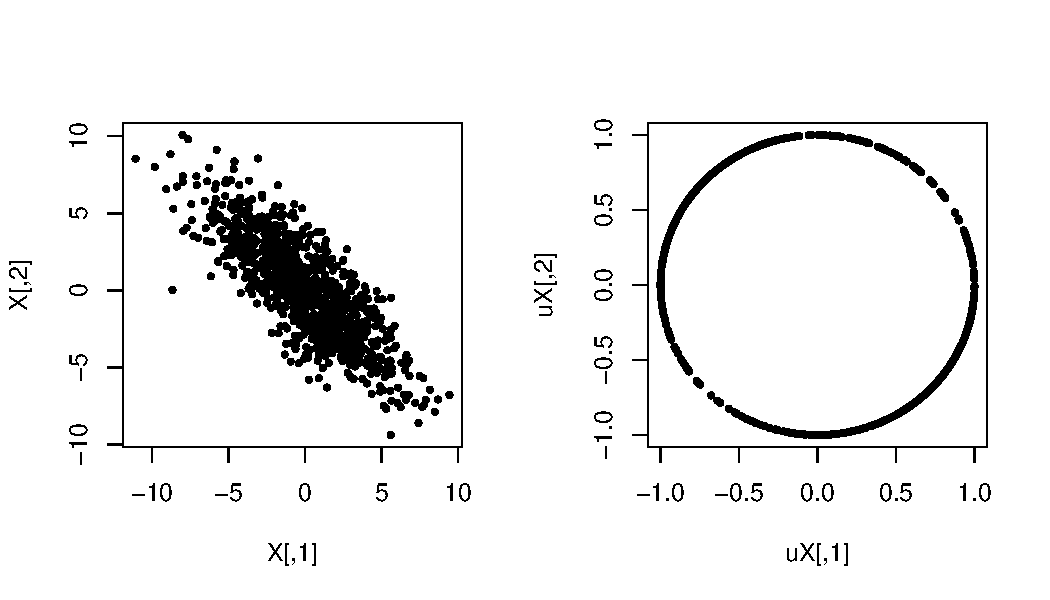
\includegraphics[height=4cm]{signs}
   \label{fig:fig2}
\end{center}\end{figure}
\end{frame}

%%%%%%%%%%%%%%%%%%%%%%%%%%%%%%%%%%%%%%%%%%%%%%%%%%%%%%%%%%%%%%%

\begin{frame}
\frametitle{Spatial ranks}

\begin{itemize}
\item Transform the original observation
%
$$
\tilde \bfx = D^- (\bfx, [\bfX] ) \bfS(\bfx - \bfmu)
$$
%
where $D^- (\bfx, [\bfX])$ is the {\colbit inverse depth} of $\bfx$: any bounded nonnegative-valued monotonically decreasing transformation on the depth function.

\vspace{1em}
This is the {\colbit Spatial Rank} of $\bfx$.

\vspace{1em}
\item Depth Covariance Matrix (DCM) $\tilde \bfSigma := \BV (\tilde \bfX) $. Has more information than spatial signs, so more efficient.
\end{itemize}

\begin{figure}\begin{center}
   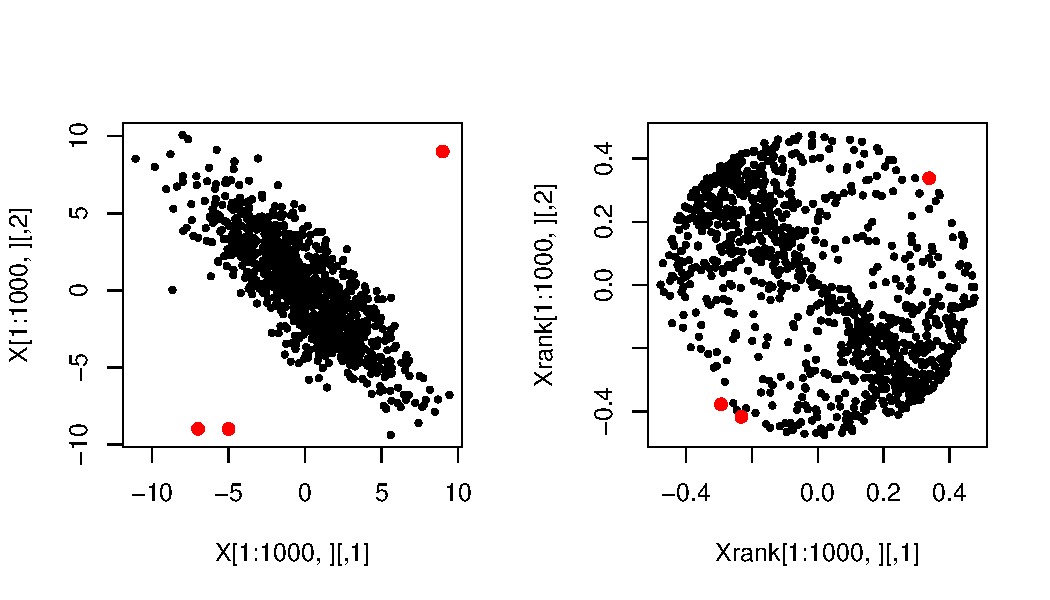
\includegraphics[height=4cm]{ranks}
   \label{fig:fig3}
\end{center}\end{figure}
\end{frame}

%%%%%%%%%%%%%%%%%%%%%%%%%%%%%%%%%%%%%%%%%%%%%%%%%%%%%%%%%%%%%%%


\begin{frame}
\frametitle{Results using spatial ranks}
\begin{itemize}
\item Recovery of population eigenvectors and eigenvalues using DCM: asymptotic and robustness properties of estimates;
\vspace{.2cm}

\item Adaptations in Sufficient Dimension Reduction and functional PCA;

\vspace{.2cm}

\item Simulations and real data applications.
\end{itemize}
\end{frame}

%%%%%%%%%%%%%%%%%%%%%%%%%%%%%%%%%%%%%%%%%%%%%%%%%%%%%%%%%%%%%%%

% Section 3: Depth-based regression
\section{Nonconvex Penalized Multitask Regression using Depth-based Penalty}

%%%%%%%%%%%%%%%%%%%%%%%%%%%%%%%%%%%%%%%%%%%%%%%%%%%%%%%%%%%%%%%

\begin{frame}
\frametitle{Penalized multitask regression}
Consider the multitask linear regression model:
%
$$ \bfY = \bfX \bfB + \bfE $$
%
where $\bfY \in \mathbb R^{n\times q}$ is the matrix of responses, and $\bfE$ is $n\times q$ the noise matrix: each row of which is drawn from $\mathcal{N}_q ({\bf 0}_q, \bfSigma)$ for a $q \times q$ positive definite matrix $\bfSigma$.

\vspace{2em}

We are interested in sparse estimates of the coefficient matrix $\bfB$ through solving penalized regression problems of the form
%
\begin{equation}\label{eqn:penEqn}
\min_\bfB \Tr \{ (\bfY - \bfX\bfB)^T ( \bfY - \bfX\bfB) \} + P_\lambda(\bfB).
\end{equation}
%

\end{frame}
%%%%%%%%%%%%%%%%%%%%%%%%%%%%%%%%%%%%%%%%%%%%%%%%%%%%%%%%%%%%%%%
\begin{frame}
\frametitle{Our estimator}
We incorporate measures of data depth as a row-level penalty function. Specifically, we estimate the coefficient matrix $\bfB$ by solving the following constrained optimization problem:
%
$$
\hat\bfB = \argmin_\bfB \left[ \Tr \{ (\bfY - \bfX\bfB)^T ( \bfY - \bfX\bfB) \} + \lambda \sum_{j=1}^p D^-( \bfb_j, F) \right]
$$
%
where $D^-( \bfx, F)$ is an inverse depth function.

\end{frame}

%%%%%%%%%%%%%%%%%%%%%%%%%%%%%%%%%%%%%%%%%%%%%%%%%%%%%%%%%%%%%%%

\begin{frame}
\frametitle{The idea}

\begin{itemize}
\item Regularization penalties can be interpreted as distance from the origin.

\item We want to use penalties that are `distance from a distribution centered at the origin'.

\item The distribution $F$ is fixed at the start of the modelling process, and can represent a prior belief on how the different responses are related among themselves.

\item Two advantages: (1) penalty attains nonconvex shape by inverting the depth function, (2) has a natural bayesian interpretation.

\item For now we assume $F$ to be spherically symmetric - plausible from a frequentist perspective.
\end{itemize}
\end{frame}

%%%%%%%%%%%%%%%%%%%%%%%%%%%%%%%%%%%%%%%%%%%%%%%%%%%%%%%%%%%%%%%

\begin{frame}
\frametitle{Simplifications}
\onslide<1->
{
\begin{itemize}
\item As $F$ to be spherically symmetric, $D^-$ becomes a function of the row-norm $r_j = \|\bfb_j\|_2$: $D^-(\bfb_j,F) = p_F(r_j)$.

\vspace{1em}
\item Use the first order Taylor approximation around a 'close enough' point $r_j^*$ instead of $p_F(r_j)$. This is local linear approximation \citep{ZouLi08}:

$$
p_F (r_j) \simeq p_F (r_j^*) + p'_F (r_j^*) ( r_j - r_j^*)
$$
\end{itemize}
}

\vspace{2em}
\onslide<2>
{
Thus the modified solution is:
$$
\hat\bfB^{(1)} = \argmin_\bfB \left[ \Tr \{ (\bfY - \bfX\bfB)^T ( \bfY - \bfX\bfB) \} + \lambda \sum_{j=1}^p p_F'(r_j^*)r_j \right]
$$

The close enough matrix $\bfB^*$ to start from can be the least squares estimate. We call this {\colbit Local Approximation by Row Norm} (LARN).
}
\end{frame}

%%%%%%%%%%%%%%%%%%%%%%%%%%%%%%%%%%%%%%%%%%%%%%%%%%%%%%%%%%%%%%%

\begin{frame}
\frametitle{Overview of work}

\begin{figure}\begin{center}
   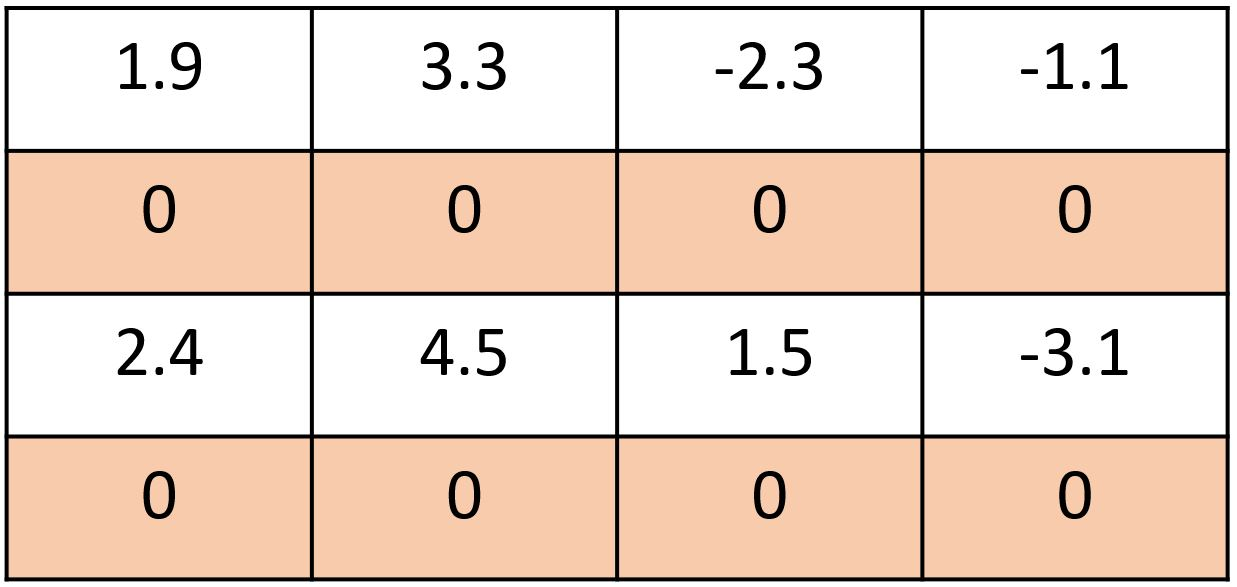
\includegraphics[height=2cm]{threspre}
   \hspace{2em}
   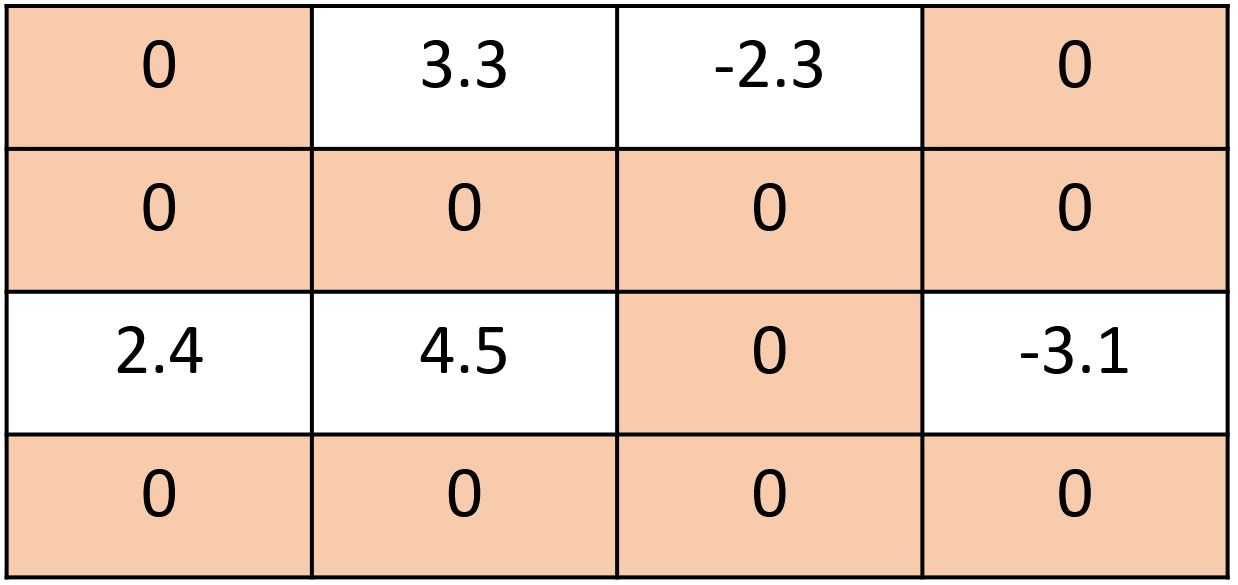
\includegraphics[height=2cm]{threspost}
   \label{fig:fig2}
\end{center}
\caption*{Pre-thresholding (L) vs. post-thresholding (R) estimators}
\end{figure}

\begin{itemize}
\item Derived theoretical properties: oracle property, near-minimax optimal performance, post-estimation thresholding to recover within row support;

\vspace{1em}
\item A block coordinate descent algorithm to compute solution;

\vspace{1em}
\item Simulation and data example.
\end{itemize}
\end{frame}


%%%%%%%%%%%%%%%%%%%%%%%%%%%%%%%%%%%%%%%%%%%%%%%%%%%%%%%%%%%%%%%

% Section 3: Depth-based model selection
\section{Generalized model discovery using statistical evaluation maps}
%%%%%%%%%%%%%%%%%%%%%%%%%%%%%%%%%%%%%%%%%%%%%%%%%%%%%%%%%%%%%%%

%\begin{frame}
%\frametitle{The motivation}
%\begin{itemize}
%\item In an regression model, the number of possible models increase excponentially: $2^p$ possible model for $p$ predictors;
%\vspace{.5em}
%\item Forward/ backward search using AIC/BIC not guaranteed to succeed. All subsets regression slow, even using efficient search strategies;
%\vspace{.5em}
%
%\item All model selection criterion are heavily based on model assumptions.
%\end{itemize}
%
%\vspace{2em}
%\noindent\textbf{Our solution}: Develop a novel model selection criterion based on data depth that works on a wide range of models, and {\colbbf selects important predictors by comparing only $p+1$ models}.
%
%\end{frame}

%%%%%%%%%%%%%%%%%%%%%%%%%%%%%%%%%%%%%%%%%%%%%%%%%%%%%%%%%%%%%%%

\begin{frame}
\frametitle{The idea}

\begin{itemize}
\item In a parametric modelling setup, any candidate model is a subset of the parameter space;
\vspace{1em}

\item We have a collection of models, and want to classify them as `good' or `bad' based on if they match with a baseline model with respect to a predefined criterion;
\vspace{1em}

\item We shall compare sampling distributions of (potentially transformed) parameter estimates of a candidate model with that of a baseline model using a generic quantity called the {\colbbf $e$-value}.
\vspace{1em}

\end{itemize}
\end{frame}

%%%%%%%%%%%%%%%%%%%%%%%%%%%%%%%%%%%%%%%%%%%%%%%%%%%%%%%%%%%%%%%

\begin{frame}[fragile]
\frametitle{Implementation: a fast variable selection `algorithm'}

\begin{minipage}[b]{.6\textwidth}

Linear regression: $Y = \bfX \bfbeta + \epsilon$. Assume that there is a true parameter vector $\bfbeta_0$, with non-zero index set $\cS_0$.

\vspace{1em}

%\begin{enumerate}
%\item Calculate $e$-value for full model: $\hat e_{n, full}$;
%\item Drop a predictor, calculate $e$-value for the reduced model: $\hat e_{n, -j}$;
%\item Repeat for all $p$ predictors;
%\item Collect predictors dropping which causes the $e$-value to decrease:
%%
%$$
%\hat \cS_0 = \{ \hat e_{n, -j} < \hat e_{n, full} \}
%$$
%%
%Then $\BP( \hat \cS_0 = \cS_0) \stackrel{P}{\raro} 1$.
%\end{enumerate}

\begin{enumerate}
\item Get $\hat \bfbeta$. Obtain its bootstrap distribution: $[\hat \bfbeta]$;

\item Replace the $j$-th coefficient with 0, name it $\hat \bfbeta_{-j}$. Do the same for its bootstrap distribution, say $[\hat \bfbeta_{-j}]$. Repeat for all $j$;

\item $e$-value of $j$-th covariate = mean depth of $\hat \bfbeta_{-j}$ with respect to $[ \hat \bfbeta]$, i.e. $\BE D( \hat \bfbeta_{-j}, [ \hat \bfbeta])$;

\item Select covariates with $e$-value less than mean depth of full model:
%
$$
\hat \cS_0 = \left\{ j: \BE D( \hat \bfbeta_{-j}, [ \hat \bfbeta]) < \BE D( \hat \bfbeta, [ \hat \bfbeta]) \right\}
$$
%
\end{enumerate}

Then $\BP (\hat \cS_0 = \cS_0 ) \raro 1$ as $n \raro \infty$.

\end{minipage}
\hspace{1.5em}
%
\tikzstyle{mybox} = [draw=black, fill=none, thick, 
rectangle, rounded corners, inner sep=.5em, inner ysep=.5em,font=\scriptsize,text width=.25\textwidth]
\begin{tikzpicture}
\node [mybox](box){%
%
\begin{minipage}{1\textwidth}
	\begin{Verbatim}[commandchars=\\\{\}]
   DroppedVar        Cn
\textbf{1         - x2 0.2356008}
\textbf{2         - x3 0.2428004}
\textbf{3         - x4 0.2448785}
\textbf{4         - x1 0.2473548}
\textbf{5         - x5 0.2486610}
\textbf{6       - x20 0.2503475}
7     <none> 0.2505000
8          - x9 0.2522873
9        - x21 0.2538186
10      - x22 0.2547132
11      - x14 0.2548410
12      - x17 0.2554293
13      - x13 0.2559990
14      - x10 0.2564211
15      - x24 0.2566334
16      - x19 0.2568725
17      - x25 0.2573902
18        - x8 0.2578656
19      - x16 0.2588032
20      - x12 0.2590218
21        - x6 0.2595048
22      - x23 0.2598039
23      - x15 0.2605307
24      - x11 0.2606763
25      - x18 0.2610460
26        - x7 0.2613168
	\end{Verbatim}
\end{minipage}
};
\end{tikzpicture}
\end{frame}

%%%%%%%%%%%%%%%%%%%%%%%%%%%%%%%%%%%%%%%%%%%%%%%%%%%%%%%%%%%%%%%

\begin{frame}
\frametitle{Why it works}
\begin{figure}
\centering
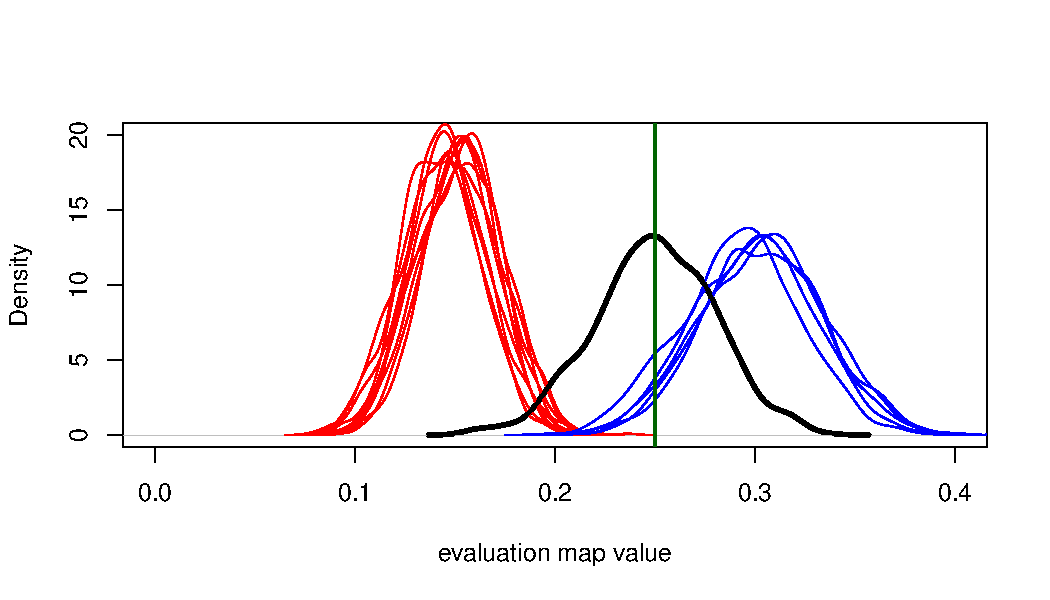
\includegraphics[width=.8\textwidth]{fullplot3}
\end{figure}

\begin{enumerate}
\item Start with full model;

\item Drop an essential predictor $\Rightarrow$ Model becomes wrong $\Rightarrow$ $e$-value shifts to left;

\item Drop a non-essential predictor $\Rightarrow$ Model still correct but nested within full model $\Rightarrow$ $e$-value shifts to right.
\end{enumerate}
\end{frame}

%%%%%%%%%%%%%%%%%%%%%%%%%%%%%%%%%%%%%%%%%%%%%%%%%%%%%%%%%%%%%%%%

\begin{frame}
\centering\huge
\textcolor{UniBlue}{\textbf{The framework}}
\end{frame}

%%%%%%%%%%%%%%%%%%%%%%%%%%%%%%%%%%%%%%%%%%%%%%%%%%%%%%%%%%%%%%%

\begin{frame}
\frametitle{Definition of a model}

\begin{minipage}{.35\textwidth}
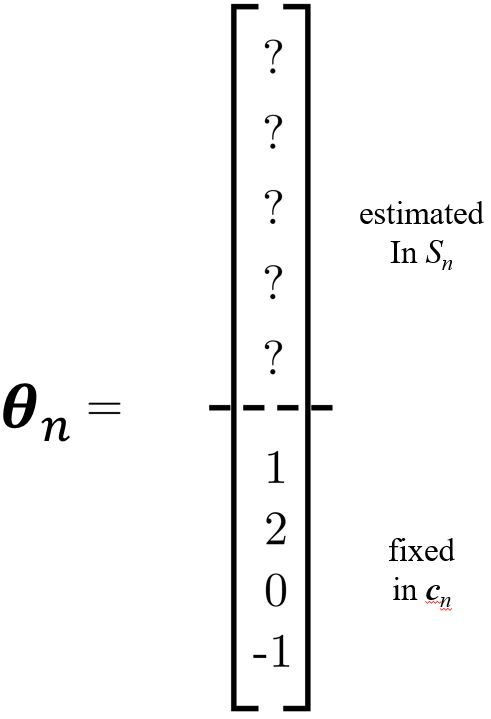
\includegraphics[width=.9\textwidth]{condmodels1}
\end{minipage}
%
\begin{minipage}{.6\textwidth}
Given traingular sequences of observable data and unknown parameters:
%
$$
\{ (\cB_n, \bftheta_n) , n \in \mathbb N \}
$$
%
$$
\cB_n = \{ B_{n1}, \ldots, B_{n k_n} \}
, \quad \bftheta_n \in \bfTheta_n \subseteq \BR^{p_n}
$$
%
a candidate model $\cM_n$ is specified by:

\vspace{1em}
\noindent\textbf{(a)} The set of indices $\cS_n \subseteq \{ 1, 2, \ldots, p_n \}$ where parameter values are {\colb estimated from the data};

\vspace{1em}
\noindent\textbf{(b)} An ordered vector of {\colb known constants} $\bfc_n = (c_{nj}: j \neq \cS_n)$ for parameters not indexed by $\cS_n$.

\vspace{1em}
Denote the model space of $\cM_n$ by $\bfTheta_{m n}$.
\end{minipage}
%
\end{frame}

%%%%%%%%%%%%%%%%%%%%%%%%%%%%%%%%%%%%%%%%%%%%%%%%%%%%%%%%%%%%%%%%


\begin{frame}
\frametitle{The preferred model}
Among all such possible models, we designate one of them as the {\colbit preferred model}: say $\cM_{* n} = (\cS_{* n}, \bfc_{* n})$.

\vspace{1em}
This is the baseline model we shall compare all models with.

\begin{example}
For variable selection, the model with all covariates is the preferred model.

\vspace{1em}
For hypothesis testing, the null model is preferred model.
\end{example}

\vspace{1em}
Designate an element of the preferred model space $\bfTheta_{* n}$ as the {\colbit preferred parameter vector} $\bftheta_{0 n}$. This is generally informative of the data generating process.
\end{frame}
%%%%%%%%%%%%%%%%%%%%%%%%%%%%%%%%%%%%%%%%%%%%%%%%%%%%%%%%%%%%%%%

\begin{frame}
\frametitle{Method of estimation}
For any candidate model $\cM_n$, we consider estimating functionals $\Psi_{s n i}(.)$ that admit an unique minimizer $\bftheta_{m n} \in \bfTheta_{m n}$:
%
$$
\Psi_{s n} (\bftheta) = \BE \sum_{i=1}^{k_n} \Psi_{s n i} (\bftheta, B_{n i});
\quad
\bftheta_{m n} = \argmin_{\bftheta \in \bfTheta_{m n}} \Psi_{s n} ( \bftheta)
$$
%
The estimate corresponding to model $\cM_n$ is obtained by minimizing its sample version:
%
$$
\hat \bftheta_{m n} = \argmin_{\bftheta \in \bfTheta_{m n}} \sum_{i=1}^{k_n} \Psi_{s n i} (\bftheta, B_{n i})
$$
%
We assume there exist $a_{s n} \uparrow \infty$ such that $[ a_{s n} (\hat \bftheta_{s n} - \bftheta_{s n}) ]$ `converges' to a distribution as $n \raro \infty$. Here $\bftheta_{s n}$ is $\bftheta_{m n}$ is $\cS_n$ indices, and same for $\hat \bftheta_{s n}$.
\end{frame}
%%%%%%%%%%%%%%%%%%%%%%%%%%%%%%%%%%%%%%%%%%%%%%%%%%%%%%%%%%%%%%%

\begin{frame}
\frametitle{A common transformation}
Now we map parameters from the parameter space to a common multivariate space using a known smooth function:
%
$$
\bfG_{m n}: \bfTheta_n \mapsto \BR^{d_n}; \quad d_n = o ( \min_s \{ a_{s n}, a_{* n} \} )
$$
%

This is for easy comparison of different kinds of modelling methods.

\begin{example} Want to compare the following models built on data $\{ (y_i, X_{1i}, X_{2i}): i = 1, \ldots, n \}$:

\vspace{1em}
\textit{(1) Linear regression} - $\quad Y_i = X_{1 i} \beta_1 + X_{2 i} \beta_2 + \epsilon_i, \epsilon_i \sim N(0, \sigma^2), \sigma > 0$;

\textit{(2) Semiparametric regression} - $\quad Y_i = X_{1 i} \beta_1 + g(X_{2 i}) + \epsilon_i$ for unknown $g$;

\textit{(3) Single index model} - $\quad Y_i = h(X_{1 i} \beta_1 + X_{2 i} \beta_2) + \epsilon_i$ for unknown $h$;

\vspace{1em}
Comparing all model in terms of prediction errors has a clearer interpretation.
\end{example}
\end{frame}
%%%%%%%%%%%%%%%%%%%%%%%%%%%%%%%%%%%%%%%%%%%%%%%%%%%%%%%%%%%%%%%

\begin{frame}
\frametitle{`Good' and `bad' models}
For $\bfg \in \BR^{d_n}$ and $\cG_n' \subseteq \BR^{d_n}$ define the following:
%
$$ d( \bfg, \cG_n') := \inf_{ \bfg' \in \cG_n'} \| \bfg - \bfg' \| $$
%

Then

\vspace{1em}
\noindent\textbf{(a)} For two sequences of models, say $\{ \cM_{1n} \}$ and $\{ \cM_{2n} \}$, we say \textit{$\{ \cM_{1n} \}$ is {\colbit nested within} $\{ \cM_{2n} \}$} if, for all sequences $\{ \bfg_{1n} : \bfg_{1n} \in \cG_{1n} \} $ we have
%
\begin{align*}\label{eq:NestedModelDef}
\lim_{n \raro \infty} d( \bfg_{1n}, \cG_{2n} ) = 0
\end{align*}
%
with $\cG_{1 n} := \{ \bfG_{m 1 n} ( \bftheta( \cM_{1 n} ) ) : \bftheta( \cM_{1 n} ) \in \bfTheta_{m 1 n} \} $ etc.

\vspace{1em}
\noindent\textbf{(b)} A sequence of models $\{ \cM_n \}$ is called {\colbit adequate} if the model $\cM_{0 n}$ corresponding to the singleton set $\bfTheta_{0 n} = \{ \bftheta_{0 n} \}$, is nested within $\cM_n$.

\vspace{1em}
\noindent\textbf{(c) }A model that is not adequate is an {\colbit inadequate model}.

\end{frame}

%%%%%%%%%%%%%%%%%%%%%%%%%%%%%%%%%%%%%%%%%%%%%%%%%%%%%%%%%%%%%%%

\begin{frame}
\frametitle{Motivation}

{\colbbf Covers obvious cases:} 
%
\begin{align*}
& (1, 2, 3, 0) \quad - \quad \text{preferred parameter vector}\\
& (*, *, *, 0) \quad - \quad \text{adequate model}\\
& (*, *, *, *) \quad - \quad \text{full model}\\
& (*, *, 0, *) \quad - \quad \text{inadequate model}
\end{align*}

\vspace{1em}
{\colbbf Covers limiting cases:}, e.g. $(*, *, *, \delta_n), \delta_n = o(1)$ will be an adequate model in our framework.
%
$$ 
$$
%

Such data generating models, e.g.
$$
Y_{ni} = X_{1i} \beta_{01} + X_{2i} \delta_n + \epsilon; \quad \beta_{01} \in \BR, \delta_n = o(1)
$$
for linear regression, frequently arise from prior choices in bayesian variable selection techniques.
\end{frame}

%%%%%%%%%%%%%%%%%%%%%%%%%%%%%%%%%%%%%%%%%%%%%%%%%%%%%%%%%%%%%%%

\begin{frame}
\frametitle{Statistical evaluation maps and $e$-values}
We now introduce an {\colbit evaluation function}:
%
$$
E_n: \BR^{d_n} \times \tilde \BR^{d_n} \mapsto [0, \infty)
$$
%
to quantify the relative position of $\hat \bfG_{m n} \equiv \bfG_{m n} ( \hat \bftheta_{m n})$ with respect to the preferred model estimate distribution. Denote this by
%
$$
E_n ( \hat \bfG_{m n}, [\hat \bfG_{* n}])
$$

{\colbbf $e$-value} is simply a functional of the distribution of this random evaluation function. Denote this by $e_n (\cM_n)$.

\vspace{1em}
We shall now elaborate on the following choice of the $e$-value:
%
$$
e_n (\cM_n) = \BE E_n ( \hat \bfG_{m n}, [\hat \bfG_{* n}])
$$

\end{frame}
%%%%%%%%%%%%%%%%%%%%%%%%%%%%%%%%%%%%%%%%%%%%%%%%%%%%%%%%%%%%%%%

%\begin{frame}
%\frametitle{$p$-values as a special case}
%
%\end{frame}

%%%%%%%%%%%%%%%%%%%%%%%%%%%%%%%%%%%%%%%%%%%%%%%%%%%%%%%%%%%%%%%

%
\begin{frame}
\centering\huge
\textcolor{UniBlue}{\textbf{Results}}
\end{frame}

%%%%%%%%%%%%%%%%%%%%%%%%%%%%%%%%%%%%%%%%%%%%%%%%%%%%%%%%%%%%%%%

\begin{frame}
\frametitle{Result: model adequacy and $e$-values}

\begin{theorem}
Under some regularity conditions, as $n \raro \infty$:
%
\begin{enumerate}
\item For the preferred model $e_n (\cM_{* n} ) \raro e_*< \infty$;
\item For any adequate model, $| e_n (\cM_n ) - e_n (\cM_{* n} ) | \raro 0$;
\item For any inadequate model, $ e_n (\cM_n ) \raro 0$.
\end{enumerate}
\end{theorem}
\end{frame}

%%%%%%%%%%%%%%%%%%%%%%%%%%%%%%%%%%%%%%%%%%%%%%%%%%%%%%%%%%%%%%%

\begin{frame}
\frametitle{A generic model selection recipe}

\begin{figure}
\centering
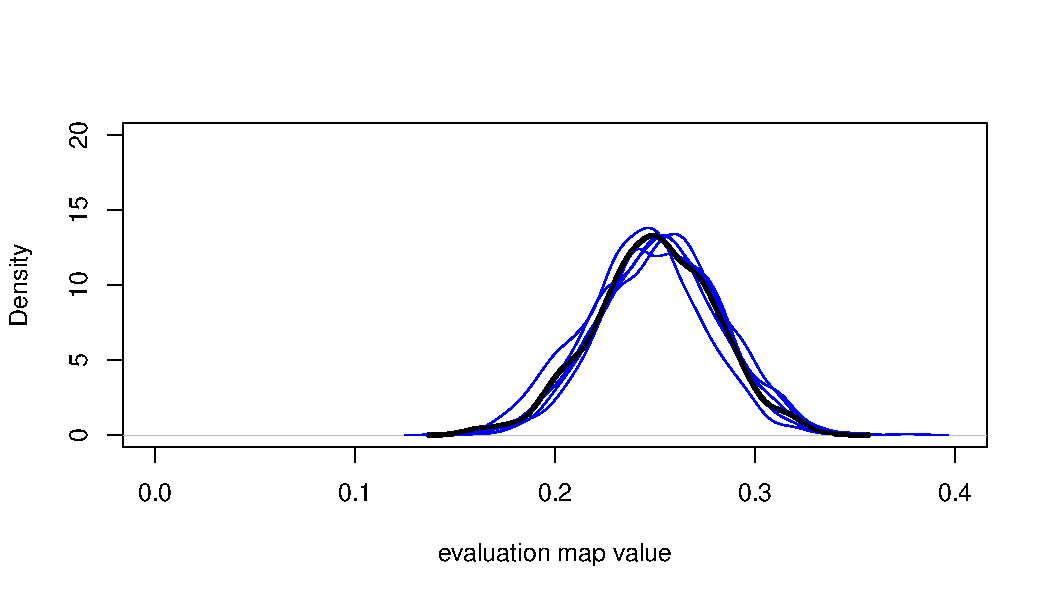
\includegraphics[width=.9\textwidth]{fullplot1}
\end{figure}
For large enough $n$, $e$-values for all adequate models will be close to that of the preferred model.

\end{frame}

%%%%%%%%%%%%%%%%%%%%%%%%%%%%%%%%%%%%%%%%%%%%%%%%%%%%%%%%%%%%%%%%

\begin{frame}
\frametitle{A generic model selection recipe}

\begin{figure}
\centering
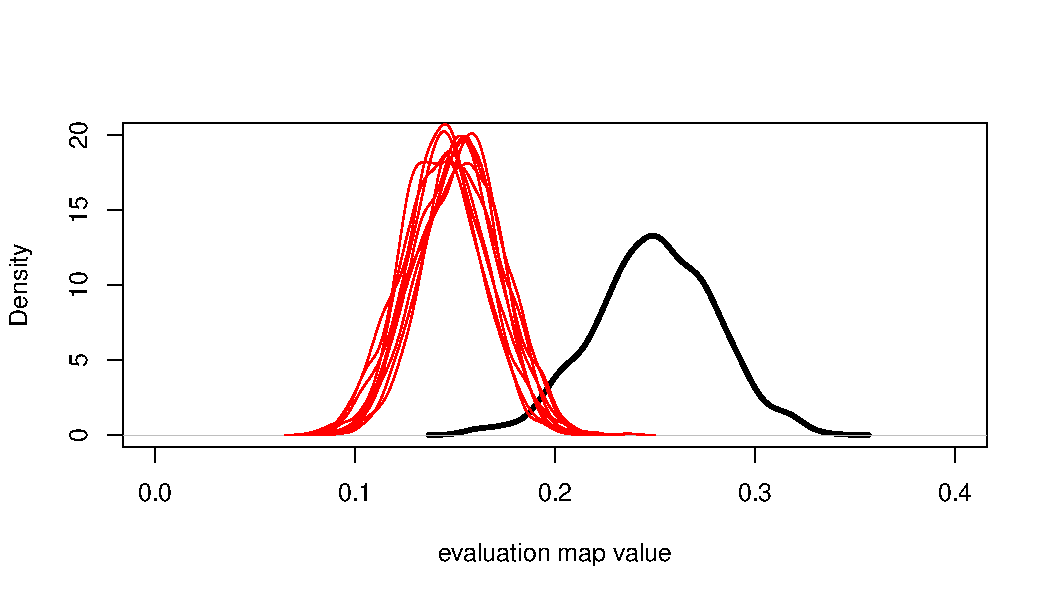
\includegraphics[width=.9\textwidth]{fullplot}
\end{figure}

But $e$-values of all inadequate models will be very small.

\end{frame}

%%%%%%%%%%%%%%%%%%%%%%%%%%%%%%%%%%%%%%%%%%%%%%%%%%%%%%%%%%%%%%%%

\begin{frame}

\begin{figure}
\centering
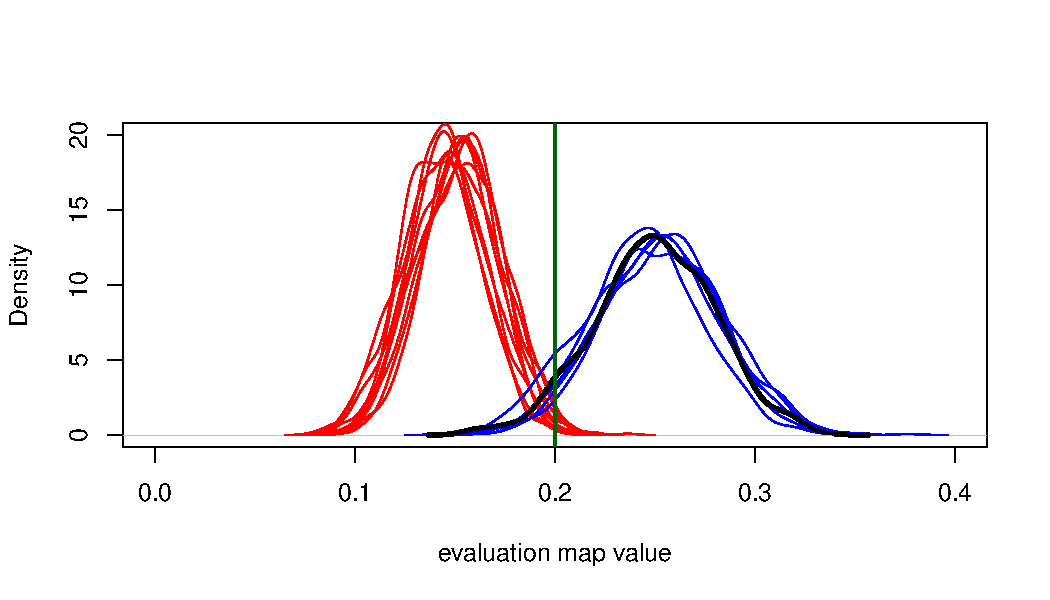
\includegraphics[width=.9\textwidth]{fullplot2}
\end{figure}

Thus we can choose an appropriate threshold $\epsilon_n$ such that any model with $e$-value below that threshold is inadequate, but $e$-value above the threshold implies the model is adequate.
\end{frame}

%%%%%%%%%%%%%%%%%%%%%%%%%%%%%%%%%%%%%%%%%%%%%%%%%%%%%%%%%%%%%%%%

\begin{frame}
\frametitle{Bootstrap estimation of $e$-values}
We shall use bootstrap to generate multiple copies of the preferred model estimate and thus approximate $[ \hat \bfG_{* n}]$.

Under standard regularity conditions \citep{ChatterjeeBose05}, we shall calculate the bootstrap estimate $\hat \bftheta_{r m n}$ by solving
%
$$
\hat \bftheta_{r m n} = \argmin_{ \bftheta \in \bfTheta_{m n}} \sum_{i=1}^{k_n} \BW_{r s n i} \Psi_{s n i} (\bftheta, B_i) 
$$
%
where $\BW_{r s n i}$ are i.i.d. weights chosen independently from the data satisfying:
\begin{eqnarray*}
\BE \BW_{r s n 1}  & = 1\\
\BV \BW_{r s n 1}  & = \tau_{s n}^{2} \uparrow \infty\\
\tau_{s n}^{2} 
%& = o ( \{min} ( a_{m n}^{2}, k_{n})), 
& = o ( a_{s n}^{2}), 
\label{eq:TauSqCondition}\\
\BE \BW_{r s n 1} \BW_{r s n 2} & = O (k_{n}^{-1}), 
\label{eq:c11} \\
\BE \BW_{r s n 1}^{2} \BW_{r s n 2}^{2} & \raro 1, 
\label{eq:c22} \\
\BE \BW_{r s n 1}^{4} & < \infty. 
\label{eq:c22}
\end{eqnarray*}

This is the {\colbit Generalized bootstrap}.
\end{frame}

%%%%%%%%%%%%%%%%%%%%%%%%%%%%%%%%%%%%%%%%%%%%%%%%%%%%%%%%%%%%%%%%

\begin{frame}
\frametitle{Result: bootstrap estimation of $e$-values}

\begin{theorem}
Suppose
%
$$
\hat e_n (\cM_n) =  \BE_r E_n (\hat \bfG_{r m n}, [\hat \bfG_{r_1 * n}])
$$
%
based on two independent sets of bootstrap samples.

Then for the above bootstrap scheme, as $n \raro \infty$:
%
\begin{enumerate}
\item For any adequate model, $| \hat e_n (\cM_n ) - \hat e_n (\cM_{* n} ) | \stackrel{P_n}{\raro} o_P (1)$;
\item For any inadequate model, $ \hat e_n (\cM_n ) \stackrel{P_n}{\raro} o_P (1)$.
\end{enumerate}
%
where $P_n$ is probability conditional on the data.
\end{theorem}

\end{frame}

%%%%%%%%%%%%%%%%%%%%%%%%%%%%%%%%%%%%%%%%%%%%%%%%%%%%%%%%%%%%%%%%

\begin{frame}
\frametitle{Fast bootstrap approximation of coefficient estimates}

The bootstrap sample is related to the actual estimate through score vectors and hessian matrices:
%
$$
\hat \bftheta_{r s n} = \hat \bftheta_{s n} - 
 \frac{\tau_{s n}}{a_{s n}} 
 \left[ \sum_{i=1}^{k_n} \Psi''_{s n i} (\hat \bftheta_{s n}, B_i) \right]^{-1/2}
\sum_{i=1}^{k_n} W_{r s n i} \Psi'_{s n i} (\hat \bftheta_{s n}, B_i) + \bfR_n
$$
%
with $\BE_r \| \bfR_n \|^2 = o_P(1)$ and $W_{r s n i} := (\BW_{r s n i} - 1)/ \tau_{s n}$.

\vspace{1em}
This means we can compute $\hat \bftheta_{r s n}$ just by generating Monte-Carlo samples and reusing other model objects. This makes the bootstrap procedure very fast.
\end{frame}

%%%%%%%%%%%%%%%%%%%%%%%%%%%%%%%%%%%%%%%%%%%%%%%%%%%%%%%%%%%%%%%%

\begin{frame}
\frametitle{A plug-in model estimate}
Start with the preferred model estimate $\hat \bftheta_{* n} = (\hat \theta_{* n 1}, \ldots, \hat \theta_{* n p_n})^T$. For any model $\cM_n$, define $\hat \bftheta_{m n}$ as:
%
$$
 \hat{\bftheta}_{m n j} = \left\{ \begin{array}{ll}
 \text{ Estimated} \ \hat{\theta}_{*n j} & \text{ for } 
 			j \in \cS_{n}; \\
 \text{ Known} \  c_{nj} & \text{ for } j \notin \cS_{n}.
\end{array}
\right.
$$
%

We shall work with these plugin estimates. This saves time while still ensuring consistency of all model estimates.

\vspace{1em}
Same for bootstrap versions:
%
$$
 \hat{\bftheta}_{r m n j} = \left\{ \begin{array}{ll}
 \text{ Estimated} \ \hat{\theta}_{r *n j} & \text{ for } 
 			j \in \cS_{n}; \\
 \text{ Known} \  c_{nj} & \text{ for } j \notin \cS_{n}.
\end{array}
\right.
$$
%
\end{frame}

%%%%%%%%%%%%%%%%%%%%%%%%%%%%%%%%%%%%%%%%%%%%%%%%%%%%%%%%%%%%%%%%%

\begin{frame}
\frametitle{Feature selection with data depth}

Now take fixed $p \equiv p_n$, and drop subscripts in $\cM_n, \cM_{* n}$ etc. Take $E_n = D$, a depth function, and the full model as preferred model. Then

\begin{theorem}
For two nested models: $\cM_{1}$ nested within $\cM_{2}$, we have $e_n (\cM_{1}) > e_n ( \cM_{2})$ for large enough $n$.
\end{theorem}

\vspace{1em}
Notice now that all adequate models are by definiton nested within the preferred model. So $e_n (\cM_*) < e_n (\cM)$ for any adequate model. Thus for large enough $n$, we can take threshold $\epsilon_n = e_n (\cM_*)$ now.

%
\begin{align*}
& (1, 2, 3, 0) \quad - \quad \text{preferred parameter vector}\\
& (*, *, *, 0) \quad - \quad \text{adequate model}\\
& (*, *, *, *) \quad - \quad \text{full model}
\end{align*}

\end{frame}

%%%%%%%%%%%%%%%%%%%%%%%%%%%%%%%%%%%%%%%%%%%%%%%%%%%%%%%%%%%%%%%%

\begin{frame}
\frametitle{One-step variable selection}
\begin{figure}
\centering
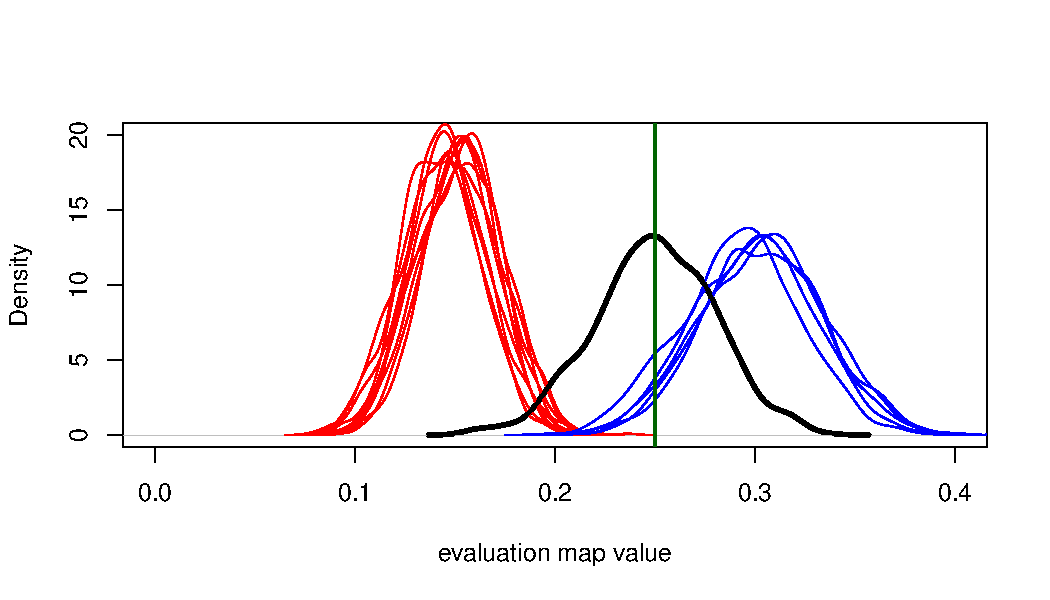
\includegraphics[width=.8\textwidth]{fullplot3}
\end{figure}

\begin{enumerate}
\item Start with full model;

\item Drop an essential predictor $\Rightarrow$ Model becomes inadequate $\Rightarrow$ $e$-value shifts to left;

\item Drop a non-essential predictor $\Rightarrow$ Model still adequate but nested within full model $\Rightarrow$ $e$-value shifts to right.
\end{enumerate}
\end{frame}

%%%%%%%%%%%%%%%%%%%%%%%%%%%%%%%%%%%%%%%%%%%%%%%%%%%%%%%%%%%%%%%%

\begin{frame}
\centering\huge
\textcolor{UniBlue}{\textbf{Numerical studies and data applications}}
\end{frame}

%%%%%%%%%%%%%%%%%%%%%%%%%%%%%%%%%%%%%%%%%%%%%%%%%%%%%%%%%%%%%%%%

\begin{frame}
\frametitle{Simulation: linear mixed models}

\begin{align*}
& \bfY_i = \bfX_i \bfbeta + \bfepsilon \in \BR^{n_i} \\
& \bfepsilon \sim N ({\bf 0}, \bfV_i) ; \quad \bfV_i = \sigma^2 \bfI_{n_i} + \bfZ_i \Delta \bfZ_i^T
\end{align*}

\begin{itemize}
\item $m$ subjects, $n_i$ observations per subject, $n = m \times n_i$ total observations;

\item $p = 9, \bfbeta = (1,1,0,0,0,0,0,0,0)^T$;

\item Elements of $\bfX_1, \ldots, \bfX_m$ chosen from Unif$(-2,2)$, random effect design matrix $\bfZ_i$ is first 4 columns of $\bfX_i$;

\item
%
$$ \Delta = \left(
	\begin{tabular}{cccc}
		9 & ~ & ~ & ~\\
		4.8 & 4 & ~ & ~\\
		0.6 & 1 & 1 & ~\\
		0 & 0 & 0 & 0\\
	\end{tabular}
	\right) $$
%
\item Two settings: (i) $m = 30, n_i=5$, (ii) $m = 60, n_i = 10$;

\item We use i.i.d. draws of Gamma(1,1) as bootstrap weights $W_i+1$.

\end{itemize}

\end{frame}
%%%%%%%%%%%%%%%%%%%%%%%%%%%%%%%%%%%%%%%%%%%%%%%%%%%%%%%%%%%%%%%%

\begin{frame}
\frametitle{Simulation results}

\begin{table}[t]
	\centering
	\begin{scriptsize}
   \begin{tabular}{lr|lll|lll}
    \hline
    Method      & Tuning     & FPR\% & FNR\% & Model size & FPR\% & FNR\% & Model size \\ \cline{3-8}
    ~ & ~ & \multicolumn{3}{l|}{$n_i=5,m=30$} & \multicolumn{3}{l}{$n_i=10,m=60$}\\ \hline
  $e$-value based       & $\tau_n / \sqrt n = 1$      & 57.4     & 0.0   & 5.24       & 43.8     & 0.0   & 4.03       \\
    ~      & $2$      & 30.4     & 0.0   & 3.32       & 12.3     & 0.0   & 2.42       \\
    ~      & $3$      & 15.6     & 0.0   & 2.54       & 3.2      & 0.0   & 2.10       \\
    ~      & $4$      & 7.3      & 0.0   & 2.24       & 1.0      & 0.0   & 2.03       \\
    ~      & $5$      & 3.0     & 0.0   & 2.09       & 0.7   & 0.0   & 2.02       \\
    ~      & $6$      & 1.7     & 0.0   & 2.05       & 0.3   & 0.0   & 2.01       \\
    ~      & $7$      & 1.0   & 0.0   & 2.03       & 0.0   & 0.0   & 2.00       \\
    ~      & $8$      & 0.7   & 0.0   & 2.02       & 0.0   & 0.0   & 2.00       \\
    ~      & $9$      & 0.0   & 0.0   & 2.00       & 0.0   & 0.0   & 2.00       \\
    ~      & $10$      & 0.0   & 0.0   & 2.00       & 0.0   & 0.0   & 2.00       \\
     \hline
    \cite{PengLu12} & BIC    & 21.5  & 9.9   & 2.26       & 1.5   & 1.9   & 2.10       \\
    ~      & AIC    & 17    & 11.0  & 2.43       & 1.5   & 3.3   & 2.20       \\
    ~      & GCV    & 20.5  & 6     & 2.30       & 1.5   & 3     & 2.18       \\
    ~      & $\sqrt{\log n/n}$ & 21    & 15.6  & 2.67       & 1.5   & 4.1   & 2.26       \\ \hline
    \end{tabular}
    \caption*{Comparison between our method and that proposed by \cite{PengLu12} through average false positive percentage, false negative percentage and model size}
    \label{table:simtable1}
    \end{scriptsize}
\end{table}
%

\end{frame}
%%%%%%%%%%%%%%%%%%%%%%%%%%%%%%%%%%%%%%%%%%%%%%%%%%%%%%%%%%%%%%%%

\begin{frame}
\frametitle{Simulation results}

\begin{table}[t]
	\centering
	\begin{scriptsize}
    \begin{tabular}{llll}
    \hline
    Method          & $\tau_n / \sqrt n$ & Setting 1 & Setting 2 \\ \hline
    $e$-value based     & 1 & 2         & 16       \\
    ~               & 2 & 36      & 67        \\
    ~               & 3 & 60        & 91      \\
    ~               & 4 & 80        & 97      \\
    ~               & 5 & 91        & 98       \\
    ~               & 6 & 95      & 99       \\
    ~               & 7 & 97       & 100       \\
    ~               & 7 & 98       & 100       \\
    ~               & 8 & 100       & 100       \\
    ~               & 10 & 100       & 100       \\\hline
    \cite{BondellKrishnaGhosh10} & ~ & 73        & 83        \\
    \cite{PengLu12}         & ~ & 49        & 86        \\
    \cite{FanLi12}           & ~ & 90        & 100       \\ \hline
    \end{tabular}
    \caption*{Comparison of our method and three sparsity-based methods of mixed effect model selection through accuracy of selecting correct fixed effects}
	\label{table:simtable2MS}
    \end{scriptsize}
\end{table}
\end{frame}

%%%%%%%%%%%%%%%%%%%%%%%%%%%%%%%%%%%%%%%%%%%%%%%%%%%%%%%%%%%%%%%%

\begin{frame}
\frametitle{Data analysis: spatial dependency in fMRI visual task data}

\begin{minipage}{.75\textwidth}

\begin{figure}
\centering
\includegraphics[width=.8\textwidth]{{"fmri image"}.png}
\end{figure}
\end{minipage}
%
\begin{minipage}{.24\textwidth}
Dimensions of 3D voxel array

$64 \times 64 \times 33$
\end{minipage}

\vspace{1em}
\begin{itemize}
\item Data collected from 19 subjects, each of which were shown two types of pictures at certain time points within a test period \citep{WakemanHenson15}.

\item Each subject went through 9 runs. In each run 210 images of their brain were recorded in 2-second intervals.

\item We use the data from a single run on subject 1, and perform a voxelwise analysis to {\colb find
out the effect of time lags and activation of neighboring voxels on the activation of each voxel}.
\end{itemize}
\end{frame}

%%%%%%%%%%%%%%%%%%%%%%%%%%%%%%%%%%%%%%%%%%%%%%%%%%%%%%%%%%%%%%%%

%\begin{frame}
%\frametitle{Model 1: temporal model}
%$$ y_i(t) = x_{ia}(t) \beta_{ia} + x_{ib}(t) \beta_{ib} + \sum_{l=1}^q t^{l-1} \gamma_{il} + \sum_{K=1}^5 y_i(t-k) \delta_{i,t-k} + \epsilon_i(t)
%$$
%
%\begin{itemize}
%\item Voxel index $i$, time index $t$;
%
%\item $x_{ia}, x_{i b}$ are stimulus values for the two types of tasks: calculated through a deterministic equation;
%
%\item $t^{l-1} \gamma_{il}$ are the polynomial drift terms quantifying background noise;
%
%\item Time dependency quantifies by the autoregressive terms $y_i(t-k) \delta_{i,t-k}$;
%
%\item We set an AR(5) structure and quadratic drift ($q=2$) and fit linear models for each voxel. Following this we run $e$-value based variable selection on all terms.
%
%\item Less than $0.1\%$ voxels were selected for each predictor, and in no particular pattern: {\colb indicating lack of temporal dependence}.
%\end{itemize}
%\end{frame}

%%%%%%%%%%%%%%%%%%%%%%%%%%%%%%%%%%%%%%%%%%%%%%%%%%%%%%%%%%%%%%%%

\begin{frame}
\frametitle{Spatial regression model}
%
\begin{align*}
y_i(t) & = x_{ia}(t) \beta_{ia} + x_{ib}(t) \beta_{ib} + \sum_{l=1}^q t^{l-1} \gamma_{il} + \sum_{n \in N_i} y_n(t) \delta_{i,n} + \epsilon_i(t) \\
& = \tilde \bfx_i (t)^T \bftheta_i + \epsilon_i (t)
\end{align*}
%

\begin{itemize}
\item Want to quantify effect of immediate neighbors: $N_i$ the set of neighbors of $i$-th voxel;

\vspace{1em}
\item Edge or corner voxels excluded: so 26 neighbors for a voxel, thus total 30 predictors.

\vspace{1em}
\item  We estimate the set of non-zero coefficients in $\bftheta_i$ using our method. Suppose this set is $R_i$, and its subsets corresponding to neighbor and non-neighbor (i.e. stimuli and drift) terms are $S_i$ and $T_i$, respectively.
\end{itemize}

\end{frame}

%%%%%%%%%%%%%%%%%%%%%%%%%%%%%%%%%%%%%%%%%%%%%%%%%%%%%%%%%%%%%%%%

\begin{frame}
\frametitle{Spatial regression model}
%
To quantify the effect of neighbors we now calculate the corresponding $F$-statistic:
%
$$
F_i = \frac{(\sum_{n \in S_i} \tilde x_{i,n} \hat\theta_{i,n})^2}{(y_i(t) - \sum_{n \in T_i} \tilde x_{i,n} \hat\theta_{i,n})^2} \frac{|n-T_i|}{|S_i|}
$$
and obtain its $p$-value, i.e. $P(F_i \geq F_{|S_i|,|n-T_i|})$.


\end{frame}

%%%%%%%%%%%%%%%%%%%%%%%%%%%%%%%%%%%%%%%%%%%%%%%%%%%%%%%%%%%%%%%%

\begin{frame}
\begin{figure}
\centering
\captionsetup{font=footnotesize}
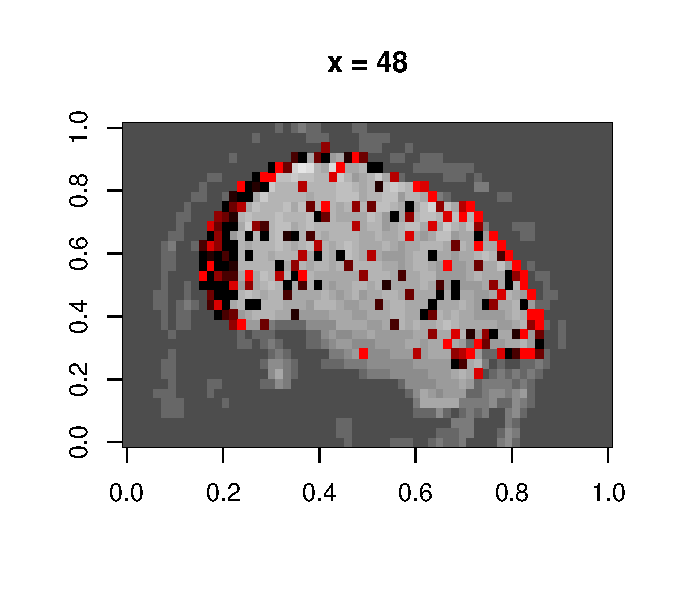
\includegraphics[width=.32\textwidth]{xslice}
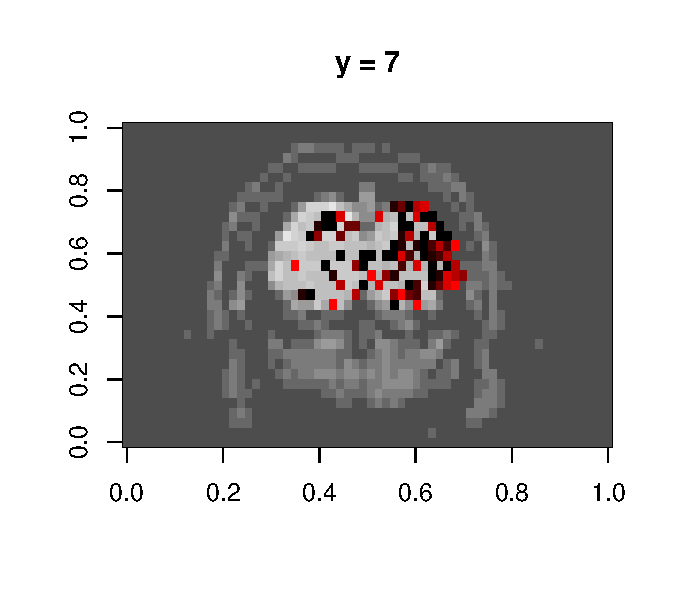
\includegraphics[width=.32\textwidth]{yslice}\\
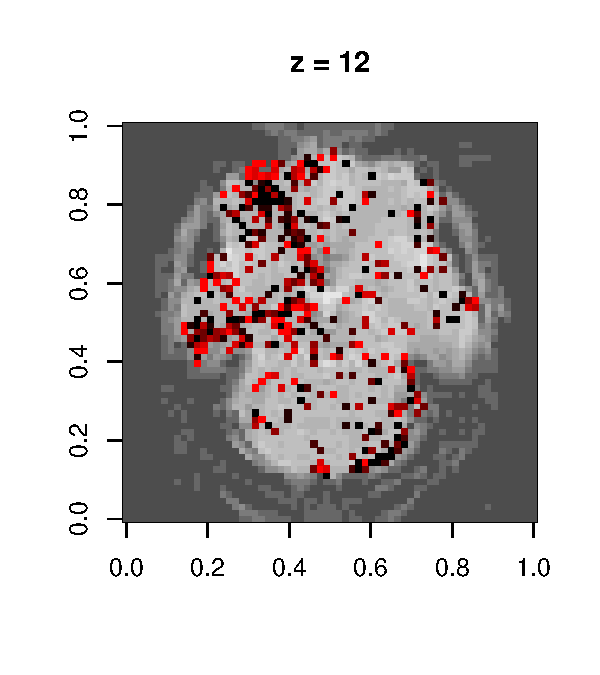
\includegraphics[width=.32\textwidth]{zslice}
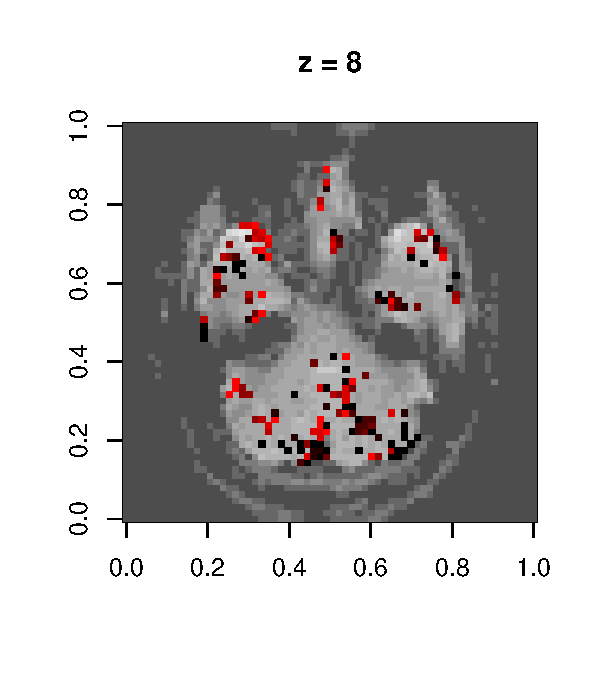
\includegraphics[width=.32\textwidth]{zslice2}\\

\caption*{Plot of significant $p$-values at $\alpha=0.05$ at specified cross-sections}

\end{figure}
\end{frame}

%%%%%%%%%%%%%%%%%%%%%%%%%%%%%%%%%%%%%%%%%%%%%%%%%%%%%%%%%%%%%%%%

\begin{frame}

\begin{figure}
\centering
\captionsetup{font=footnotesize}
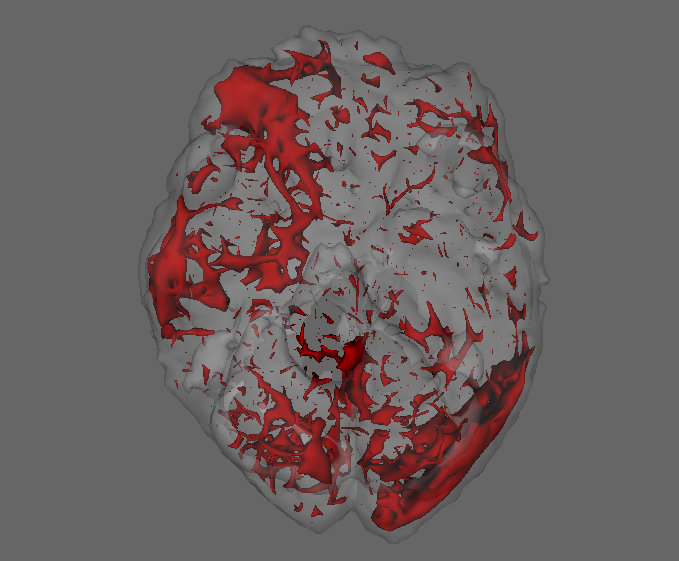
\includegraphics[width=.5\textwidth]{screenshot}
\caption*{A smoothed surface obtained from the $p$-values clearly shows high spatial dependence in right optic nerve, auditory nerves, auditory cortex and left visual cortex areas as well as Cerebellum}
\end{figure}
\end{frame}

%%%%%%%%%%%%%%%%%%%%%%%%%%%%%%%%%%%%%%%%%%%%%%%%%%%%%%%%%%%%%%%%

% Section 4: Twin studies SNP selection
\section{Selecting important SNPs from multi-SNP mixed models on Twin Studies GWAS data}

%%%%%%%%%%%%%%%%%%%%%%%%%%%%%%%%%%%%%%%%%%%%%%%%%%%%%%%%%%%%%%%%

\begin{frame}
\frametitle{Motivation}

Genome-Wide Association Studies (GWAS) based on families are used in behavioral genetics to control for environmental variation, thus requiring smaller sample size to detect Single Nucleotide Polymorphisms (SNP) responsible behind traits like alcoholism and drug addiction, and also to quantify gene-environment interaction.

\vspace{1em}
Two challenges:

\begin{enumerate}
\item SNPs highly correlated, weak signals of individual SNPs;

\item Need to use mixed models to account for within-family dependence.
\end{enumerate}

\end{frame}

%%%%%%%%%%%%%%%%%%%%%%%%%%%%%%%%%%%%%%%%%%%%%%%%%%%%%%%%%%%%%%%%

\begin{frame}
\frametitle{Statistical model}
%
\begin{align*}
& \bfY_i = \alpha + \bfG_i \bfbeta_g + \bfC_i \bfbeta_c + \bfepsilon_i\\
& \bfepsilon_i \sim \cN_{n_i} ({\bf 0}, \bfV_i); \quad \bfV_i = \sigma_a^2 \bfPhi_i + \sigma_c^2 {\bf 1} {\bf 1}^T + \sigma_e^2 \bfI_{n_i}
\end{align*}
%

\begin{itemize}

\item Total $m$ families, with the $i$-th pedigree containing $n_i$ individuals;

\vspace{1em}
\item $\bfY_i = (y_{i 1}, \ldots, y_{i n_i})^T $ are the quantitative trait values for individuals in $i$-th pedigree, $\bfG_i \in \BR^{ n_i \times p_s}$ containing their genotypes for a bunch of SNPs, $\bfC_i \in \BR^{ n_i \times p}$ contain the data on individual-specific covariates;

\vspace{1em}
\item Three variance components correspond to polygenic effect due to other SNPs, shared environment effect and individual-specific effects. This is called the {\colbbf ACE model}.

\end{itemize}

\end{frame}
%%%%%%%%%%%%%%%%%%%%%%%%%%%%%%%%%%%%%%%%%%%%%%%%%%%%%%%%%%%%%%%%

\begin{frame}
\frametitle{The relationship matrix $\bfPhi_i$}
%
\begin{minipage}{.63\textwidth}
%
\begin{align*}
& \bfPhi_{MZ} = \begin{bmatrix}
1 & 0 & 1/2 & 1/2 \\
0 & 1 & 1/2 & 1/2 \\
1/2 & 1/2 & 1 & 1\\
1/2 & 1/2 & 1 & 1
\end{bmatrix},\\
& \bfPhi_{DZ} = \begin{bmatrix}
1 & 0 & 1/2 & 1/2 \\
0 & 1 & 1/2 & 1/2 \\
1/2 & 1/2 & 1 & 1/2\\
1/2 & 1/2 & 1/2 & 1
\end{bmatrix},\vspace{1em}
\\
& \bfPhi_{Adopted} = \bfI_4
\end{align*}
%
\end{minipage}
%
\begin{minipage}{.34\textwidth}
$\bfPhi_i$ depends on the type of the $i$-th family:

\vspace{1em}

MZ = family with identical or monozygous twins,

DZ = family with identical or dizygous twins.

\end{minipage}

\end{frame}
%%%%%%%%%%%%%%%%%%%%%%%%%%%%%%%%%%%%%%%%%%%%%%%%%%%%%%%%%%%%%%%%

\begin{frame}{Objective}
Want to detect the non-zero entries of $\bfbeta_g$ in the above model.

\vspace{1em}
State-of-the-art is to perform single-SNP analysis and then correct for multiple testing. This loses power. We want to use the \textbf{$e$-values} method to improve that.
\end{frame}

%%%%%%%%%%%%%%%%%%%%%%%%%%%%%%%%%%%%%%%%%%%%%%%%%%%%%%%%%%%%%%%%

\begin{frame}
\frametitle{A new $e$-value}
{\colbbf Problem: weak signal of individual SNPs}

\begin{minipage}{.64\textwidth}
\begin{figure}
\centering
\includegraphics[height=.4\textheight]{{"plot_h0.05_tau2"}.pdf}\\
\includegraphics[height=.4\textheight]{{"plot_h0.05_tau4"}.pdf}\\
\label{fig:figSmallhSim}
\end{figure}
\end{minipage}
%
\begin{minipage}{.34\textwidth}
Using means as $e$-values makes the procedure very conservative.

\vspace{1em}
But it may still be possible to use a tail quantile to distinguish between distributions.
\end{minipage}

\end{frame}

%%%%%%%%%%%%%%%%%%%%%%%%%%%%%%%%%%%%%%%%%%%%%%%%%%%%%%%%%%%%%%%%

\begin{frame}
\frametitle{A new $e$-value}

We now take as $e$-value the $q$-th quantile of the evaluation map distribution, for some fixed $q \in (0,1)$. Under slightly stronger assumptions than before, all results go through for a general evaluation map in the population and bootstrap worlds.


\vspace{1em}
\begin{enumerate}
\item Estimate the full model coefficient, say $\hat \bfbeta_g \equiv \hat \bfbeta$ (by R package \texttt{regress} )

\item Obtain its bootstrap distribution: $[\hat \bfbeta]$;

\item Replace the $j$-th coefficient with 0, name it $\hat \bfbeta_{-j}$. Do the same for its bootstrap distribution, say $[\hat \bfbeta_{-j}]$. Repeat for all $j$;

\item $e$-value of $j$-th covariate = tail probability of the $q$-th quantile of $[ E (\hat \bfbeta_{-j}, [ \hat \bfbeta]) ]$ with respect to $[ E (\hat \bfbeta, [ \hat \bfbeta]) ]$;

\item Select $j$-th covariate if its $e$-value is less than $t q$, for some $0<t<1$.
\end{enumerate}

\end{frame}

%%%%%%%%%%%%%%%%%%%%%%%%%%%%%%%%%%%%%%%%%%%%%%%%%%%%%%%%%%%%%%%%

\begin{frame}{Simulation setup}
\begin{itemize}
\item 250 pedigrees, each of size 4: consisting of parents and MZ twins;
\item $\alpha = 0$, no environmental covariates;
\item 50 SNPs in correlated blocks of 6,4,6,4 and 30: MAF of SNPs in the blocks 0.2, 0.4, 0.4, 0.25 and 0.25;
\item $\sigma^2_a = 4, \sigma^2_c = 1, \sigma^2_e = 1$;
\item First SNP of first 4 blocks are causal: each having heritability (a measure of magnitude of non-zero effect) $h/6 \%$;
\item Full setup replicated 1000 times.

\vspace{1em}
\item Methods compared:\\
{\colb mBIC2} - Variant of BIC that control false discovery rate at 0.05;\\
{\colb RFGLS} - Fast method of fitting single-SNP ACE models. Do Benjamini-Hochberg correction on $p$-values to control FDR at 0.05.
\end{itemize}
\end{frame}
%%%%%%%%%%%%%%%%%%%%%%%%%%%%%%%%%%%%%%%%%%%%%%%%%%%%%%%%%%%%%%%%

\begin{frame}
\frametitle{Simulation results}

\begin{table}
\begin{scriptsize}
\centering
    \begin{tabular}{c|c|c|c|cccc}
    \hline
    6x    & mBIC2       & RFGLS  & \multicolumn{5}{|c}{quantile $e$-values}    \\\cline{4-8}
    Heritability    &           & +BH		 & $q$    & $t=0.8$     & $t=0.7$     & $t=0.6$     & $t=0.5$     \\
    \hline
    ~    & ~         & ~         & 0.9      & 0.95/0.97 & 0.95/0.97 & 0.95/0.98 & \textbf{0.94/0.98} \\
    $h=10$ & 0.79/0.99 & 0.95/0.92 & 0.5      & 0.96/0.97 & 0.96/0.98 & 0.95/0.98 & 0.94/0.98 \\
    ~    & ~         & ~         & 0.2      & 0.96/0.94 & 0.96/0.97 & 0.95/0.97 & 0.95/0.98 \\\hline
    ~    & ~         & ~         & 0.9      & 0.72/0.95 & 0.7/0.96  & 0.69/0.96 & \textbf{0.66/0.97} \\
    $h=5$  & 0.41/0.99 & 0.62/0.97 & 0.5      & 0.78/0.94 & 0.75/0.94 & 0.72/0.95 & 0.71/0.96 \\
    ~    & ~         & ~         & 0.2      & 0.83/0.91 & 0.78/0.94 & 0.75/0.95 & 0.73/0.95 \\\hline
    ~    & ~         & ~         & 0.9      & 0.26/0.97 & 0.24/0.97 & 0.23/0.98 & \textbf{0.21/0.98} \\
    $h=2$  & 0.11/0.99 & 0.14/0.99 & 0.5      & 0.34/0.95 & 0.28/0.96 & 0.27/0.97 & 0.26/0.97 \\
    ~    & ~         & ~         & 0.2      & 0.46/0.91 & 0.34/0.95 & 0.3/0.96  & 0.27/0.96 \\\hline
    ~    & ~         & ~         & 0.9      & 0.12/0.98 & 0.1/0.98  & 0.09/0.99 & \textbf{0.08/0.99} \\
    $h=1$  & 0.05/0.99 & 0.04/0.99    & 0.5      & 0.16/0.96 & 0.13/0.97 & 0.12/0.97 & 0.11/0.98 \\
    ~    & ~         & ~         & 0.2      & 0.25/0.93 & 0.16/0.96 & 0.13/0.97 & 0.13/0.97 \\\hline
    ~    & ~         & ~         & 0.9      & --/0.99 & --/0.99 & --/0.99 & \textbf{--/0.99}    \\
    $h=0$  & --/0.99 & --/0.99       & 0.5      & --/0.98 & --/0.98 & --/0.99 & --/0.99 \\
    ~    & ~         & ~         & 0.2      & --/0.94 & --/0.98 & --/0.98 & --/0.99 \\\hline
    \end{tabular}
\end{scriptsize}
\caption*{Average true positive/ true negative detection proportions over 1000 replications}
\end{table}
\end{frame}
%%%%%%%%%%%%%%%%%%%%%%%%%%%%%%%%%%%%%%%%%%%%%%%%%%%%%%%%%%%%%%%%

\begin{frame}
\frametitle{Simulation results}

% latex table generated in R 3.3.2 by xtable 1.8-2 package
% Sun Apr 16 18:24:09 2017
% latex table generated in R 3.3.2 by xtable 1.8-2 package
% Sun Apr 16 18:24:48 2017
\begin{table}
\begin{scriptsize}
\centering
    \begin{tabular}{c|c|c|c|cccc}
    \hline
    6x    & mBIC2       & RFGLS  & \multicolumn{5}{|c}{quantile $e$-values}    \\\cline{4-8}
    Heritability    &           & +BH		 & $q$    & $t=0.8$     & $t=0.7$     & $t=0.6$     & $t=0.5$     \\ \hline
    ~    & ~         & ~         & 0.9      & 0.96/0.97 & 0.96/0.97 & 0.95/0.98 & \textbf{0.94/0.98} \\
    $h=10$ & 0.84/0.99 & 0.96/0.99 & 0.5      & 0.96/0.97 & 0.96/0.97 & 0.95/0.98 & 0.95/0.98 \\
    ~    & ~         & ~         & 0.2      & 0.97/0.95 & 0.96/0.97 & 0.96/0.97 & 0.95/0.98 \\\hline
    ~    & ~         & ~         & 0.9      & 0.73/0.95 & 0.71/0.95 & 0.7/0.96  & \textbf{0.67/0.97} \\
    $h=5$  & 0.48/0.99 & 0.64/0.99 & 0.5      & 0.79/0.93 & 0.76/0.94 & 0.73/0.95 & 0.72/0.95 \\
    ~    & ~         & ~         & 0.2      & 0.85/0.91 & 0.79/0.93 & 0.76/0.94 & 0.74/0.95 \\\hline
    ~    & ~         & ~         & 0.9      & 0.29/0.96 & 0.27/0.97 & 0.25/0.98 & \textbf{0.23/0.98} \\
    $h=2$  & 0.16/0.99 & 0.16/0.99    & 0.5      & 0.37/0.95 & 0.31/0.96 & 0.3/0.96  & 0.29/0.97 \\
    ~    & ~         & ~         & 0.2      & 0.53/0.91 & 0.38/0.95 & 0.33/0.95 & 0.3/0.96  \\\hline
    ~    & ~         & ~         & 0.9      & 0.15/0.97 & 0.13/0.98 & 0.12/0.98 & \textbf{0.10/0.99}  \\
    $h=1$  & 0.08/0.99 & 0.05/0.99    & 0.5      & 0.2/0.96  & 0.17/0.97 & 0.15/0.97 & 0.13/0.98 \\
    ~    & ~         & ~         & 0.2      & 0.35/0.93 & 0.21/0.96 & 0.17/0.97 & 0.16/0.97 \\\hline
    ~    & ~         & ~         & 0.9      & --/0.97 & --/0.98 & --/0.98 & \textbf{--/0.99} \\
    $h=0$  & --/0.98 & --/0.99    & 0.5      & --/0.95 & --/0.97 & --/0.97 & --/0.98 \\
    ~    & ~         & ~         & 0.2      & --/0.90 & --/0.95 & --/0.97 & --/0.97 \\\hline
    \end{tabular}
\caption*{Average true positive/ true negative detection proportions over 1000 replications: true positive = can detect any SNP in the same block}
\end{scriptsize}
\end{table}
\end{frame}
%%%%%%%%%%%%%%%%%%%%%%%%%%%%%%%%%%%%%%%%%%%%%%%%%%%%%%%%%%%%%%%%

\begin{frame}{Analyzing the Minnesota Twin Studies data}

\begin{itemize}
\item Analyze data on families with MZ twins: 682 families;

\item Response variable: amount of alcohol consumption;

\item Look at models specific to well-studied genes for alcoholism: GABRA2, ADH1B,
ADH1C, SLC6A3, SLC6A4, OPRM1, CYP2E1, DRD2, ALDH2, and COMT;

\item Group together ADH genes as individual genes have very small number of SNPs. Also do SLC6A4+DRD2 together as they are known to interact with each other.

\item We take $q=0.9, t=0.5$ to increase specificity, i.e. detection of true negatives.
\end{itemize}
\end{frame}
%%%%%%%%%%%%%%%%%%%%%%%%%%%%%%%%%%%%%%%%%%%%%%%%%%%%%%%%%%%%%%%%

\begin{frame}
\frametitle{Number of detected SNPs}

\begin{table}[t]
\begin{footnotesize}
\centering
\begin{tabular}{c|c}
    \hline
    Gene   & Total/detected \\
    ~      & SNP            \\  \hline
GABRA2 &  11/5 \\ 
  ADH &  21/5 \\ 
  SLC6A3 &  18/4 \\ 
  SLC6A4 &   5/0 \\ 
  OPRM1 &  46/29 \\
  CYP2E1 &   9/5 \\ 
  DRD2 &  17/0 \\ 
  ALDH2 &   5/5 \\ 
  COMT &  15/9 \\  
  SLC6A4 + DRD2 & 22/0 \\\hline
\end{tabular}
\caption*{Table of analyzed genes and detected SNPs in them}
\end{footnotesize}
\end{table}
\end{frame}

%%%%%%%%%%%%%%%%%%%%%%%%%%%%%%%%%%%%%%%%%%%%%%%%%%%%%%%%%%%%%%%%

\begin{frame}{GABRA2}

\begin{figure}
\includegraphics[width=.9\textwidth]{{"plotGABRA2"}.pdf}
\end{figure}

Detects rs1808851 and rs279856, which have very high correlation with the well-known rs279858. This was missed by a previous analysis \citep{IronsThesis12}.
\end{frame}

%%%%%%%%%%%%%%%%%%%%%%%%%%%%%%%%%%%%%%%%%%%%%%%%%%%%%%%%%%%%%%%%

\begin{frame}{ADH genes}

\begin{figure}
\includegraphics[width=.9\textwidth]{{"plotADH"}.pdf}
\end{figure}

Detects rs13103626 and rs10516430 at positions 99317251 and 99337881 in chr 4: close to the well-known rs1229984 at position 99318162.

\end{frame}
%%%%%%%%%%%%%%%%%%%%%%%%%%%%%%%%%%%%%%%%%%%%%%%%%%%%%%%%%%%%%%%%

\begin{frame}
\frametitle{Conclusion and future work}

In this thesis, I have proposed several methods of using depths or depth-like quantities in traditional statistical inference, e.g. PCA, sparse regression, model selection.

\vspace{1em}
Future works include:

\begin{enumerate}
\item Formulation of depth in a general Hilbert space;

\item Exploring different uses of the $e$-values framework: for example in multiple testing;

\item Extension of the signed rank and depth-based penalization framework.
\end{enumerate}
\end{frame}

%%%%%%%%%%%%%%%%%%%%%%%%%%%%%%%%%%%%%%%%%%%%%%%%%%%%%%%%%%%%%%%%

\begin{frame}
\frametitle{References}

{\scriptsize
\bibliographystyle{plainnat}
\bibliography{finalbib}
}
\end{frame}

%%%%%%%%%%%%%%%%%%%%%%%%%%%%%%%%%%%%%%%%%%%%%%%%%%%%%%%%%%%%%%%%

\begin{frame}
\frametitle{Acknowledgements}

\begin{itemize}
\item Anshu Chatterjee;

\vspace{1em}
\item Saonli Basu;

\vspace{1em}
\item Lan Wang, Xiaotong Shen, Gongjun Xu;

\vspace{1em}
\item NSF grant IIS-1029711, U of M Interdisciplinary Doctoral Fellowship;

\vspace{1em}
\item Abhirup Mallik, Adam Maidman, Daniel Eck, Sakshi Arya and other School of Statistics students;

\vspace{1em}
\item Faculty and staff of the School of Statistics.
\end{itemize}
\end{frame}
%%%%%%%%%%%%%%%%%%%%%%%%%%%%%%%%%%%%%%%%%%%%%%%%%%%%%%%%%%%%%%%%

\begin{frame}
\centering\huge
\textcolor{UniBlue}{\textbf{THANK YOU!}}
\end{frame}


%\begin{frame}
%\frametitle{Conditional models}
%
%\begin{minipage}{.6\textwidth}
%Consider the general estimation problem
%%
%$$\bfy = h(X\bfbeta) + \bfepsilon $$
%%
%Assume $h(.)$ to be known, and $\bfepsilon$ having an arbitrary error distribution.
%
%\vspace{1em}
%In this setup, a candidate model can be uniquely identified as $\bfbeta$ whose some indices are fixed (at values $\bfbeta_c$) and others (indices $\alpha$) are unknown.
%\vspace{1em}
%
%We say this combination is a {\colbbf conditional model}:
%$$ \mu = (\alpha, \bfbeta_c) $$
%\end{minipage}
%%
%\begin{minipage}{.35\textwidth}
%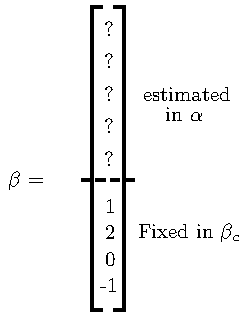
\includegraphics[width=\textwidth]{condmodels}
%\end{minipage}
%\end{frame}
%
%%%%%%%%%%%%%%%%%%%%%%%%%%%%%%%%%%%%%%%%%%%%%%%%%%%%%%%%%%%%%%%%
%
%\begin{frame}
%\frametitle{More on conditional models}
%
%\begin{outline}
%\1 The set of all possible conditional models is:
%%
%$$ \mathcal{M}_c = \left\{(\alpha, \bfbeta_c): \alpha \subseteq \mathcal{I}_p, \bfbeta_c \in \mathbb{R}^{|\mathcal{I}_p \backslash \alpha|} \right\} $$
%%
%with $\mathcal{I}_p = \{ 1,2,...,p \}$.
%\vspace{1em}
%
%\1 \textbf{Correct conditional models} are conditional models such that
%$\bfbeta_c$ is a subvector of $\bfbeta$, made from its elements at indices NOT in $\alpha$, i.e. $\mathcal{I}_p \backslash \alpha$;
%\vspace{1em}
%
%\1 \textbf{Wrong conditional models} are conditional models such that
%	\2 At least one element of $\bfbeta_c$ is not in $\bfbeta$; \\
%	\2 Or $\bfbeta_c$ is a subvector of $\bfbeta$, but not at indices $\mathcal{I}_p \backslash \alpha$.
%\vspace{1em}
%
%\1 \textbf{Nested conditional models}: Given two conditional models $\mu^1 = (\alpha^1, \bfbeta^1_c)$ and $\mu^2 = (\alpha^2, \bfbeta^2_c)$, $\mu^2$ is said to be nested in $\mu^1$ if:
%	\2 $\alpha^2 \supseteq \alpha^1$;
%	\2 $\bfbeta^2_c$ is a subvector of $\bfbeta^1_c$, at indices $\alpha^2 \backslash \alpha^1$.
%\end{outline}
%\end{frame}
%
%%%%%%%%%%%%%%%%%%%%%%%%%%%%%%%%%%%%%%%%%%%%%%%%%%%%%%%%%%%%%%%%
%
%\begin{frame}
%\frametitle{Defining the selection criterion}
%Now consider estimators $\hat \bfbeta_n$ obtained from a sample of sizw $n$ that have sampling distributions that are asymptotically elliptical, with mean $\bfbeta$ and covariance matrix $V_n$, such that
%\vspace{1em}
%
%\noindent\textbf{(1)} $\{V_n\}$ is a sequence of positive-definite matrices such that $V_p - V_q$ is positive definite for all $p<q$;
%
%\noindent\textbf{(2)} There exists a positive definite matrix $V$ such that $\text{plim}_{n \rightarrow \infty} (n V_n) = V$.
%\vspace{2em}
%
%Given a conditional model $\mu$, estimate $\bfbeta$ at indices $\alpha$ and append that by $\bfbeta_c$ to obtain a $p$-dimensional estimate of $\bfbeta$: part fixed, part random. Denote this by $\tilde\bfbeta_n (\mu)$.
%
%Then our selection criterion is defined as:
%%
%$$ C_n (\mu) = \mathbb{E}_{F_n | \mu} \left[ D \left( \tilde\bfbeta_n (\mu), F_n \right) \right] $$
%\end{frame}
%
%%%%%%%%%%%%%%%%%%%%%%%%%%%%%%%%%%%%%%%%%%%%%%%%%%%%%%%%%%%%%%%%
%
%\begin{frame}
%\frametitle{The master theorem}
%\begin{Theorem}
%Consider the sets of correct conditional models ($\mathcal{M}_c^c$) and wrong conditional models ($\mathcal{M}_c^w$), and estimators $\hat\bfbeta_n$ satisfying properties mentioned before. Then:
%
%\begin{enumerate}
%\item For a wrong conditional model $\mu^w \in \mathcal{M}_c^w$, $C_n(\mu^w) \rightarrow 0$ as $n \rightarrow \infty$;
%\item For a correct conditional model $\mu^c \in \mathcal{M}_c^c$, $C_n(\mu^c) = C(\mu^c)$ for all values of $n$, $C(\mu^c) \geq 0$ being only dependent on $\mu^c$;
%\item For a sequence of nested correct conditional models, say $\mu^c_1, ... , \mu^c_k$; $k \leq p$ and any $n$, we shall have
%%
%$$ C_n (\mu^c_1) \geq \ldots \geq C_n(\mu^c_k) $$
%%
%\end{enumerate}
%\end{Theorem}
%\end{frame}
%
%%%%%%%%%%%%%%%%%%%%%%%%%%%%%%%%%%%%%%%%%%%%%%%%%%%%%%%%%%%%%%%%
%
%%\begin{frame}
%%\frametitle{The one-step algorithm}
%%\begin{enumerate}
%%\item Obtain $C_n(\mu_{\text{full}}^c)$; set $i=1$;
%%
%%\item Drop the predictor with index $i$, obtain $C_n$ for that model, say $\mu_{\text{full}-i}$;
%%
%%\item Repeat step 2 for $i=2,...,p$, covering all predictors;
%%
%%\item Collect the predictors dropping which causes a decrease in $C_n$:
%%%
%%$$ \alpha_0^n = \left\lbrace i: C_n(\mu_{\text{full}-i}) < C_n(\mu_{\text{full}}^c) \right\rbrace $$
%%%
%%\item When $n$ is large enough so that $C_n(\mu_{\text{full}-i}) < C_n(\mu_{\text{full}}^c)$ for all $i \in \alpha_0$, we shall have $\alpha_0^n = \alpha_0$.
%%\end{enumerate}
%%\end{frame}
%
%%%%%%%%%%%%%%%%%%%%%%%%%%%%%%%%%%%%%%%%%%%%%%%%%%%%%%%%%%%%%%%%
%
%\begin{frame}
%\frametitle{Estimating $C_n$}
%The master theorem is essentially a population level result. In a sample setup we neither know multiple instances of $\tilde\bfbeta_n (\mu)$, nor of $\hat\bfbeta_n$ (for getting hold of $F_n$).
%\vspace{1em}
%
%So we use bootstrap to get both. Thus $C_n(\mu)$ is estimated by:
%%
%$$ \hat C_n(\mu) = \mathbb E_b \left[ D \left( \tilde \bfbeta_n^b(\mu), F_n^{b_1} \right) \right] $$
%%
%where $b$ and $b_1$ denote the collections of random sample weights for  the two \textit{independent} bootstrap samples.
%\vspace{1em}
%
%The two separate bootstraps are required for theoretical tractability.
%\end{frame}
%
%%%%%%%%%%%%%%%%%%%%%%%%%%%%%%%%%%%%%%%%%%%%%%%%%%%%%%%%%%%%%%%%
%
%\begin{frame}
%\frametitle{Bootstrap asymptotics for correct conditional models: assumptions}
%
%\begin{small}
%\noindent\textbf{(i) Differentiability:} The depth function $D(.,.)$ is Gateaux differentiable in its second argument. The functional derivative of the depth at any point $\bfx$ with respect to a probability distribution $P$ is the influence function for any point $\bfz \in \mathbb{R}^p$:
%%
%$$ IF( \bfz; D(\bfx, P), P ) = \lim_{\epsilon \downarrow 0} \frac{D(\bfx, P) - D(\bfx, (1-\epsilon)P + \epsilon \delta_\bfz)}{\epsilon} $$
%%
%where $\delta_\bfz$ is the probability distribution that has point mass at $\bfz$. 
%
%\vspace{1em}
%\noindent\textbf{(ii) Continuity:}
%
%\noindent\textbf{(A)} For sequences of probability distributions $P_n$ and $Q_n$, both taking values in $\mathbb{R}^p$, $P_n \leadsto Q_n$ implies that
%%
%$$ \sup_{\bfb \in \mathbb{R}^p} | D( \bfb, P_n) - D(\bfb, Q_n) | \rightarrow 0 \text{ as } n \rightarrow \infty $$
%%
%\noindent\textbf{(B)} For a probability distribution $P$ taking values in $\mathbb{R}^p$, and points $\bfx, \bfy \in \mathbb{R}^p$,
%%
%$$ | D(\bfx, P) - D(\bfy, P) | \leq M \| \bfx - \bfy \| $$
%%
%for some constant $M > 0$.
%\end{small}
%\end{frame}
%
%%%%%%%%%%%%%%%%%%%%%%%%%%%%%%%%%%%%%%%%%%%%%%%%%%%%%%%%%%%%%%%%
%
%\begin{frame}
%\frametitle{Bootstrap asymptotics for correct conditional models: result}
%
%\begin{small}
%\begin{Theorem}
%Consider bootstrap schemes $b, b_1$ and a depth function $D$ satisfying above assumptions such that the following hold, for some $\{ t_n \} \uparrow \infty$ such that $\{n/t_n\} \uparrow \infty$:
%%
%\begin{enumerate}
%\item $\sqrt {n/t_n} (\hat \bfbeta_n^{b_1} - \hat \bfbeta_n )$ and $\sqrt {n/t_n} (\hat \bfbeta_n^{b} - \hat \bfbeta_n )$ both converge to the same elliptical distribution, with mean ${\bf 0}_p$ and covariance matrix $V$;
%
%\item The limit $\lim_{n\rightarrow\infty}\sigma^2_n(b,b_1)/ m_n$ exists, where:
%%
%$$ \sigma^2_n(b,b_1) = \mathbb E_b \mathbb{E}_{b_1} \left[ IF \left( \bfd_{nb_1}; D \left( \bfd_{nb} (\mu), \hat F_n - \bfbeta \right), \hat F_n - \bfbeta \right)^2 \right]$$
%\end{enumerate}
%%
%with $\bfd_{nb} = (\hat\bfbeta_n^b - \hat\bfbeta_n)/\sqrt{t_n}, \bfd_{nb}(\mu) = (\tilde\bfbeta_n^b (\mu) - \hat\bfbeta_n)/\sqrt{t_n}$. Then, given the data for any correct conditional model $\mu$ we shall have
%%
%\begin{equation}
%\left[ \frac{\sigma_n^2(b,b_1)}{m_n} + \gamma_n^2 + \delta_n^2\right]^{-1/2} \left( \hat C_n (\mu) - C_n (\mu) \right) \leadsto N \left( 0, 1 \right)
%\end{equation}
%%
%where $\gamma_n^2$ and $\delta_n^2$ are $o_P(1)$.
%\end{Theorem}
%\end{small}
%\end{frame}
%
%%%%%%%%%%%%%%%%%%%%%%%%%%%%%%%%%%%%%%%%%%%%%%%%%%%%%%%%%%%%%%%%
%
%\begin{frame}
%\frametitle{What happens for wrong conditional models?}
%
%\begin{itemize}
%\item We fix a part of the coefficient vector, and estimate the rest. In the bootstrap world, this brings in a $O_P(1/\sqrt n)$ bias;
%\vspace{1em}
%
%\item Choosing a bootstrap scheme such that $t_n \rightarrow \infty$ is essential in letting this bias go to zero asymptotically for correct models;
%\vspace{1em}
%
%\item This does not work for wrong models. Our immediate future work is to investigate this;
%\vspace{1em}
%
%\item For now we shall do this bootstrap for wrong models as well. We will consider an ad-hoc method of bias correction, and compare outputs from both corrected and uncorrected methods.
%\end{itemize}
%\end{frame}
%
%%%%%%%%%%%%%%%%%%%%%%%%%%%%%%%%%%%%%%%%%%%%%%%%%%%%%%%%%%%%%%%%
%
%\begin{frame}
%\frametitle{Implementation through wild bootstrap}
%
%{\colubf Paired bootstrap:}
%%
%$$ \bfy_b = P_b \bfy, X_b = P_b X; \quad \text{where } P_b \text{ is a } n \times n \text{ permutatation matrix} $$
%\vspace{1em}
%
%{\colubf Residual bootstrap:}
%%
%$$ \bfy_b = \hat \bfy + P_b \hat\bfepsilon, X_b = X $$
%\vspace{1em}
%
%\begin{bclogo}{Wild bootstrap \citep{Mammen93}:}
%%
%$$ \bfy_b = \hat \bfy + U_b \hat\bfepsilon, X_b = X $$
%%
%where $U_b = \text{diag} (U_{1b},...,U_{nb})$ with the $U_{ib}$-s drawn independently from a probability distribution with mean 0, variance $\tau_n^2$.
%\end{bclogo}
%\end{frame}
%
%%%%%%%%%%%%%%%%%%%%%%%%%%%%%%%%%%%%%%%%%%%%%%%%%%%%%%%%%%%%%%%%
%
%\begin{frame}
%\frametitle{Simulation 1: setup}
%
%\begin{itemize}
%\item $n = 100, p = 10$;
%
%\item Coefficient vector $\bfbeta$ is made of $k$ ones and $p-k$ zeros: $k = 2,4,6,8$;
%
%\item Randomly chosen 100 rows and first 10 columns in the dataset available in \url{http://www.stat.umn.edu/geyer/5102/data/ex6-8.txt} taken as $X$. Responses generated as $\bfy = X\bfbeta + \bfepsilon; \bfepsilon \sim \mathcal{N}_p ( {\bf 0}_p , I_p)$;
%
%\item 1000 such samples are drawn;
%
%\item Bootstrap sample size 1000 for estimating $C_n$. Bootstrap standard deviation $\tau_n = \text{seq}(1,10, \text{by}=0.1)$;
%
%\item Compared with AIC and BIC backward deletion and all-subset regression.
%\end{itemize}
%\end{frame}
%
%%%%%%%%%%%%%%%%%%%%%%%%%%%%%%%%%%%%%%%%%%%%%%%%%%%%%%%%%%%%%%%%
%
%\begin{frame}
%\frametitle{Simulation 1: results}
%
%\begin{figure}[t]
%\captionsetup{justification=centering, font=footnotesize}
%\begin{center}
%\includegraphics[width=.9\linewidth]{simplot24}
%\label{fig:simplot1}
%\end{center}
%\end{figure}
%
%\end{frame}
%
%%%%%%%%%%%%%%%%%%%%%%%%%%%%%%%%%%%%%%%%%%%%%%%%%%%%%%%%%%%%%%%%
%
%\begin{frame}
%\frametitle{Simulation 1: results}
%
%\begin{figure}[t]
%\captionsetup{justification=centering, font=footnotesize}
%\begin{center}
%\includegraphics[width=.9\linewidth]{simplot68}
%\label{fig:simplot2}
%\end{center}
%\end{figure}
%
%\end{frame}
%
%%%%%%%%%%%%%%%%%%%%%%%%%%%%%%%%%%%%%%%%%%%%%%%%%%%%%%%%%%%%%%%%
%
%\begin{frame}
%\frametitle{Simulation 2: Synthetic data analysis}
%
%\begin{itemize}
%\item $p = 9, \bfbeta = (0,1,1,0,0,0,0,0,0,0)^T$ (length 10 including the intercept);
%\item Linear mixed model: $m$ subjects, $n_i$ observations per subject, $n = m \times n_i$ total observations;
%
%\item Elements of all but first column of $X_{n \times (p+1)} $ chosen from Unif$(-2,2)$, random effect design matrix $Z$ is first 4 columns of $X$;
%
%\item $\bfy_i = X_i \bfbeta + \bfepsilon_i $, where $\bfepsilon_i \sim \mathcal N_{n_i} ({\bf 0}, \sigma^2 I + Z_i D Z_i^T)$ with
%%
%$$ D = \left(
%	\begin{tabular}{cccc}
%		9 & ~ & ~ & ~\\
%		4.8 & 4 & ~ & ~\\
%		0.6 & 1 & 1 & ~\\
%		0 & 0 & 0 & 0\\
%	\end{tabular}
%	\right) $$
%%
%\item Two settings: (i) $m = 30, n_i=5$, (ii) $m = 60, n_i = 10$;
%
%\end{itemize}
%\end{frame}
%
%%%%%%%%%%%%%%%%%%%%%%%%%%%%%%%%%%%%%%%%%%%%%%%%%%%%%%%%%%%%%%%%
%
%\begin{frame}
%\frametitle{Simulation 2: results}
%
%\begin{table}
%	\centering
%	\begin{scriptsize}
%   \begin{tabular}{ll|lll|lll}
%    \hline
%    Method      & Tuning     & FPR\% & FNR\% & Model size & FPR\% & FNR\% & Model size \\ \cline{3-8}
%    ~ & ~ & \multicolumn{3}{l|}{$n_i=5,m=30$} & \multicolumn{3}{l}{$n_i=10,m=60$}\\ \hline
%    Depth-based      & $\tau=1$      & 60.1     & 0.0   & 5.35       & 56.7     & 0.0   & 4.96       \\
%    ~      & $\tau=2$      & 30.8     & 0.0   & 3.21       & 29.4     & 0.0   & 3.09       \\
%    ~      & $\tau=3$      & 11.1     & 0.0   & 2.37       & 9.6      & 0.0   & 2.32       \\
%    ~      & $\tau=4$      & 2.4      & 0.0   & 2.14       & 1.8      & 0.0   & 2.01       \\
%    ~      & $\tau=5$      & 1     & 0.0   & 2.03       & 0.0   & 0.0   & 2.00       \\
%    ~      & $\tau=6$      & 0.2     & 0.0   & 2.01       & 0.0   & 0.0   & 2.00       \\
%    ~      & $\tau=7$      & 0.0   & 0.0   & 2.00       & 0.0   & 0.0   & 2.00       \\
%    ~      & $\tau=8$      & 0.0   & 0.0   & 2.00       & 0.0   & 0.0   & 2.00       \\ \hline
%    \cite{PengLu12} & BIC    & 21.5  & 9.9   & 2.26       & 1.5   & 1.9   & 2.10       \\
%    ~      & AIC    & 17    & 11.0  & 2.43       & 1.5   & 3.3   & 2.20       \\
%    ~      & GCV    & 20.5  & 6     & 2.30       & 1.5   & 3     & 2.18       \\
%    ~      & $\sqrt{\log n/n}$ & 21    & 15.6  & 2.67       & 1.5   & 4.1   & 2.26       \\ \hline
%    \end{tabular}
%    \caption{Comparison between our method and that proposed by \cite{PengLu12} through average false positive percentage (FPR\%), false negative percentage (FNR\%) and model size}
%    \label{table:simtable1}
%    \end{scriptsize}
%\end{table}
%
%\end{frame}
%
%%%%%%%%%%%%%%%%%%%%%%%%%%%%%%%%%%%%%%%%%%%%%%%%%%%%%%%%%%%%%%%%
%
%\begin{frame}
%\frametitle{Simulation 2: results}
%
%\begin{table}
%	\centering
%	\begin{scriptsize}
%    \begin{tabular}{llll}
%    \hline
%    Method          & ~ & Setting 1 & Setting 2 \\ \hline
%    Depth-based     & $\tau=1$ & 1         & 1.5       \\
%    ~               & $\tau=2$ & 29.5      & 29        \\
%    ~               & $\tau=3$ & 70        & 73.5      \\
%    ~               & $\tau=4$ & 93        & 94.5      \\
%    ~               & $\tau=5$ & 97        & 100       \\
%    ~               & $\tau=6$ & 99.5      & 100       \\
%    ~               & $\tau=7$ & 100       & 100       \\
%    ~               & $\tau=8$ & 100       & 100       \\ \hline
%    \cite{BondellKrishnaGhosh10} & ~ & 73        & 83        \\
%    \cite{PengLu12}         & ~ & 49        & 86        \\
%    \cite{FanLi12}           & ~ & 90        & 100       \\ \hline
%    \end{tabular}
%    \caption{Comparison of our method and three sparsity-based methods of mixed effect model selection through accuracy of selecting correct fixed effects}
%	\label{table:simtable2}
%    \end{scriptsize}
%\end{table}
%
%\end{frame}
%
%%%%%%%%%%%%%%%%%%%%%%%%%%%%%%%%%%%%%%%%%%%%%%%%%%%%%%%%%%%%%%%%%
%%
%\begin{frame}
%\frametitle{Future work}
%
%\begin{enumerate}
%\item Theoretical results for bootstrapping wrong models;
%\vspace{.5em}
%
%\item Extending to high-dimensional regression and robust regression models:\\
%\hspace{1em}\cite{Hall09};\\
%\hspace{1em}\cite{SBVanAelst08};
%\vspace{.5em}
%
%\item Preference ordering of unidentifiable models:\\
%\hspace{1em}\cite{Yuan11}.
%\end{enumerate}
%\end{frame}
%
%%%%%%%%%%%%%%%%%%%%%%%%%%%%%%%%%%%%%%%%%%%%%%%%%%%%%%%%%%%%%%%%
%
%% Section 4: Depth-weighted regression
%\section{Iterated depth-weighted multivariate regression}
%%%%%%%%%%%%%%%%%%%%%%%%%%%%%%%%%%%%%%%%%%%%%%%%%%%%%%%%%%%%%%%%%
%
%\begin{frame}
%\frametitle{The algorithm}
%Consider the multiple linear regression setup: $Y = \bfX^T\bfbeta + \epsilon$ and the following iterated-reweighted least squares algorithm:
%
%\begin{enumerate}
%\item Set $k=1$;
%
%\item Define the starting estimate of the coefficient vector to be the least square estimate: $\hat\bfbeta^{(0)} = \hat\bfbeta$;
%
%\item Give weights to the observation: $w_i^{(k)} = D(r_i^{(k)}, F^{(k)})$ for $i=1,2,...,n$, where $r_i^{(k)} = y_i - \bfx_i^T \hat\bfbeta^{(k-1)}$ and $F^{(k)}$ is the empirical distribution function of all $e_i$'s;
%
%\item Update the coefficient estimate $\hat\bfbeta^{(i)}$ as the weighted least square solution taking weights $w_i^{(k)}$;
%
%\item Set $k \leftarrow k+1$. Repeat until convergence.
%\end{enumerate}
%\end{frame}
%
%%%%%%%%%%%%%%%%%%%%%%%%%%%%%%%%%%%%%%%%%%%%%%%%%%%%%%%%%%%%%%%%%
%
%\begin{frame}
%\frametitle{Simulations}
%
%\begin{tiny}
%\begin{table}
%	\centering
%	   \begin{tabular}{c|cccc}
%    \hline
%    \multicolumn{5}{l}{$n=50$} \\ \hline
%    Contamination & RMSE($n$,LS)  & RMSE($n$,Huber) & RMSE($n$,$D_1$)   & RMSE($n$,$D_2$) \\ \hline
%    0\%           & 0.51 & 0.52  & 0.52 & 0.68  \\
%    10\%          & 1.38 & 0.57  & 0.59 & 0.65  \\
%    20\%          & 2.69 & 1.10  & 1.34 & 0.95  \\
%    30\%          & 3.76 & 2.49  & 2.63 & 1.52  \\
%    40\%          & 3.60 & 2.63  & 2.80 & 1.91  \\ \hline
%        \multicolumn{5}{l}{$n=100$} \\ \hline
%    Contamination & RMSE($n$,LS)  & RMSE($n$,Huber) & RMSE($n$,$D_1$)   & RMSE($n$,$D_2$) \\ \hline
%    0\%           & 0.35 & 0.36  & 0.36 & 0.46  \\
%    10\%          & 1.46 & 0.45  & 0.50 & 0.49  \\
%    20\%          & 1.79 & 0.51  & 0.59 & 0.52  \\
%    30\%          & 2.52 & 0.87  & 1.09 & 0.78  \\
%    40\%          & 3.11 & 1.85  & 2.18 & 1.27  \\ \hline
%        \multicolumn{5}{l}{$n=200$} \\ \hline
%    Contamination & RMSE($n$,LS)  & RMSE($n$,Huber) & RMSE($n$,$D_1$)   & RMSE($n$,$D_2$) \\ \hline
%    0\%           & 0.24 & 0.24  & 0.24 & 0.31  \\
%    10\%          & 1.09 & 0.30  & 0.35 & 0.29  \\
%    20\%          & 1.32 & 0.38  & 0.44 & 0.35  \\
%    30\%          & 1.28 & 0.41  & 0.49 & 0.40  \\
%    40\%          & 1.65 & 0.66  & 0.80 & 0.60  \\ \hline
%        \multicolumn{5}{l}{$n=500$} \\ \hline
%    Contamination & RMSE($n$,LS)  & RMSE($n$,Huber) & RMSE($n$,$D_1$)   & RMSE($n$,$D_2$) \\ \hline
%    0\%           & 0.15 & 0.15  & 0.15 & 0.19  \\
%    10\%          & 0.51 & 0.16  & 0.18 & 0.18  \\
%    20\%          & 0.70 & 0.20  & 0.24 & 0.20  \\
%    30\%          & 0.98 & 0.30  & 0.36 & 0.29  \\
%    40\%          & 1.08 & 0.42  & 0.50 & 0.40  \\ \hline
%    \end{tabular}
%    \caption{Comparison of depth-weighted iterated estimators with least square and Huber's M-estimators of $\bfbeta = (1,2,3,4,5,6,7,8)^T$ for different degrees of contamination. $D_1$ and $D_2$ are projection depth and halfspace depths, respectively}
%	\label{table:regsimtable1}
%\end{table}
%\end{tiny}
%
%\end{frame}
%
%
%\begin{frame}
%\frametitle{References}
%{\scriptsize
%\bibliographystyle{plainnat}
%\bibliography{MSbib}
%}
%\end{frame}
%
%%%%%%%%%%%%%%%%%%%%%%%%%%%%%%%%%%%%%%%%%%%%%%%%%%%%%%%%%%%%%%%%
%
%\begin{frame}
%\centering\huge
%\textcolor{UniBlue}{\textbf{THANK YOU!}}
%\end{frame}
%
%%---------------------------------------------------
%%%%%%%%%%%%%%%%%%%%%%%%%%%%%%%%%%%%%%%%%%%%%%%%%%%%%%%%%%%%%%%%
%\appendix
%%%%%%%%%%%%%%%%%%%%%%%%%%%%%%%%%%%%%%%%%%%%%%%%%%%%%%%%%%%%%%%%
%
%\begin{frame}
%\frametitle{Application: selection of important predictors in Indian monsoon}
%
%\begin{itemize}
%\item Annual median observations for 1978-2012;
%
%\item Local measurements across 36 weather stations (e.g. elevation, latitude, longitude), as well as global variables (e.g. El-Nino, tropospheric temperature variations) : total 35 predictors;
%
%\item Aim is two-fold: (i) Selecting important predictors, (ii) providing good predictions using the reduced model.
%\end{itemize}
%\end{frame}
%
%%%%%%%%%%%%%%%%%%%%%%%%%%%%%%%%%%%%%%%%%%%%%%%%%%%%%%%%%%%%%%%%
%
%\begin{frame}
%\frametitle{Application: results}
%
%\begin{figure}[t]
%\captionsetup{justification=centering, font=footnotesize}
%\begin{center}
%\subfigure[]{\epsfxsize=0.45\linewidth \epsfbox{rolling_predbias_full_vs_reduced}}
%\subfigure[]{\epsfxsize=0.45\linewidth \epsfbox{rolling_predMSE_full_vs_reduced}}\\
%\caption{Comparing full model rolling predictions with reduced models:\\
%(a) Bias across years, (b) MSE across years}
%\label{fig:prepost1}
%\end{center}
%\end{figure}
%\end{frame}
%
%%%%%%%%%%%%%%%%%%%%%%%%%%%%%%%%%%%%%%%%%%%%%%%%%%%%%%%%%%%%%%%%
%
%\begin{frame}
%\frametitle{Application: results}
%
%\begin{figure}[t]
%	\captionsetup{justification=centering, font=footnotesize}
%	\begin{center}
%		%\subfigure[]{}
%		%\subfigure[]{}
%		\subfigure[]{\epsfxsize=0.45\linewidth \epsfbox{rolling_density2012_full_vs_reduced}}
%		\subfigure[]{\epsfxsize=0.45\linewidth \epsfbox{rolling_map2012_full_vs_reduced_cropped}}
%		\caption{Comparing full model rolling predictions with reduced models:\\
%		(a) density plots for 2012, (b) stationwise residuals for 2012}
%		\label{fig:prepost2}
%	\end{center}
%\end{figure}
%\end{frame}

%%%%%%%%%%%%%%%%%%%%%%%%%%%%%%%%%%%%%%%%%%%%%%%%%%%%%%%%%%%%%%%

\end{document}